\documentclass[12pt,a4paper, twoside, openright]{report}
\PassOptionsToPackage{T1}{fontenc}
  \usepackage{fontenc}

\PassOptionsToPackage{utf8}{inputenc}
  \usepackage{inputenc}
  %**************************************************************************
%Lingua, Font
%**************************************************************************
 \PassOptionsToPackage{italian}{babel}
 \usepackage{babel}

 %Font Computer Modern in Postscript
\usepackage{lmodern}

%**************************************************************************
%Impostazioni Bibilatex
%**************************************************************************
\usepackage{csquotes}%necessario Per Bibliografia con BibTeX
\PassOptionsToPackage{%
  backend=bibtex8,bibencoding=utf8,%
  language=auto,%
  style=numeric-comp,%
  sorting=nyt, % name, year, title
  maxbibnames=10, % default: 3, et al.
  %backref=true,%
  natbib=true % natbib compatibility mode (\citep and \citet still work)
}{biblatex}
    \usepackage{biblatex} 
%**************************************************************************
%Pagina, Tabelle
%**************************************************************************
\usepackage{layaureo}

\usepackage{geometry} %Alternativa personalizzabile a layaureo
%\geometry{a4paper, top=3cm, bottom=3cm, left= 3cm, right= 3cm} 

\usepackage{fancyhdr}%Pesonalizza stile degli Headings
\pagestyle{fancy}
\renewcommand{\chaptermark}[1]{\markboth{#1}{}}
\renewcommand{\sectionmark}[1]{\markright{ \thesection.\ #1}{}}
\renewcommand{\headrulewidth}{0.2pt}%linea superiore
\fancyhf{}
\fancyhead[LE]{\small \textsc{\leftmark}}
\fancyhead[RE,LO]{\thepage}
\fancyhead[RO]{\small\textsc{\rightmark}}

\setcounter{secnumdepth}{1}%numerati fino a
\setcounter{tocdepth}{1}%nell'indice fino a

\usepackage{tocstyle}%Impostazioni Indice
\usetocstyle{noonewithdot}%toglie i puntini 


\usepackage{indentfirst}

\PassOptionsToPackage{bottom}{footmisc}%Forza le note a fondo pagina
\usepackage{footmisc}

\usepackage{verbatim}%per grossi commenti e Codici

\PassOptionsToPackage{font=small}{caption} % ,format=hang ,labelformat=smallcaps
\usepackage{caption}

\usepackage{booktabs}
%**************************************************************************
%Pacchetti Matematici e Fisici
%**************************************************************************
 
\usepackage{amsmath}
\usepackage{amsfonts}
\usepackage{amssymb}
\usepackage{mathrsfs}
%\PassOptionToPackage{separate-uncertainty=true, output-decimal-marker={.},input-decimal-markers={.}}{siunitx}
%\usepackage{siunitx}%Pacchetto per le unità di misura

\usepackage{relsize,exscale}%fa gli integral più grandi

%**************************************************************************
%Impostazioni dei Colori
%**************************************************************************
\PassOptionsToPackage{dvipsnames}{xcolor}
\usepackage{xcolor}
 \definecolor{Ccitation}{rgb}{0,0.5,0} % WebGreen
\definecolor{Curl}{named}{Maroon} % Maroon
\definecolor{Clink}{named}{RoyalBlue} % RoyalBlue 
%**************************************************************************
%Immagini e Tikz
%**************************************************************************
\usepackage{graphicx}

\usepackage{wrapfig}%gruppi di immagini
\usepackage{subfig}

%\usepackage{tikz} %Disegni
%\usetikzlibrary{external}%
%\tikzexternalize[mode=list and make, prefix=ext-tikz/]%Crea cartella esterna per documenti
%\usepackage{pgfplots} %plottare grafici
%\pgfplotsset{compat=1.5} %impostazione necessaria per far funzionare bene pgfplot
%**************************************************************************
%References
%**************************************************************************
\usepackage{hyperref}
\hypersetup{%Collegamenti colorati per PDF
  colorlinks=true, linktocpage=true, %pdfstartpage=3,%pdf apre a pagina 3
   pdfstartview=FitV,%
  %Collegamenti in Nero per stampa
  %colorlinks=false, linktocpage=false, pdfstartpage=3, pdfstartview=FitV, pdfborder={0 0 0},%
  breaklinks=true, pageanchor=true,%
  pdfpagemode=UseNone, %
  % pdfpagemode=UseOutlines,%
  plainpages=false, bookmarksnumbered, bookmarksopen=true, bookmarksopenlevel=1,%
  hypertexnames=true, pdfhighlight=/O,%nesting=true,%frenchlinks,%
  urlcolor=Curl, linkcolor=Clink, citecolor=Ccitation,%
  pdfauthor=Lorenzo Dall'Olio,pdftitle=Funzionamento di un pulsossimetro ed analisi di serie temporali pulsossimetriche
  }
%
\usepackage[italian]{babel}
\usepackage{newlfont}
\usepackage[T1]{fontenc}
\usepackage{color}
\usepackage{mathtools}
\usepackage{amsmath,amsfonts,amssymb}
\usepackage{graphicx}
\usepackage[version=3]{mhchem}
\graphicspath{{Immagini/}}%LaTeX cerca le immagini direttamente nella cartella Immagini
\usepackage{url}
\usepackage[figurename=Fig.]{caption}
\usepackage{subfig}
\usepackage[font={small}]{caption}
\usepackage{booktabs}
\usepackage{siunitx}
\sisetup{exponent-product = \cdot, output-product = \cdot}
\usepackage[nottoc,notlot,notlof]{tocbibind}
\usepackage{floatrow}
\DeclareFloatFont{footnotesize}{\footnotesize}
\floatsetup[table]{font=footnotesize}
\usepackage{caption}
\captionsetup{skip=0pt}
\usepackage{afterpage}
\usepackage[utf8]{inputenc}
\usepackage{algorithm}
\usepackage[noend]{algpseudocode}
\usepackage{geometry}
\textwidth=450pt\oddsidemargin=0pt
\bibliography{bibliography}

\begin{document}
	%\hypersetup{
		%colorlinks,
	%	citecolor=black,
	%	filecolor=black,
	%	linkcolor=black,
	%	urlcolor=black
   	%}

\raggedbottom
\frenchspacing

\begin{titlepage}
%
%
%
%
%
\begin{center}
{{\Large{\textsc{Alma Mater Studiorum $\cdot$ Universit\`a di Bologna}}}} 
\rule[0.1cm]{15.8cm}{0.1mm}
\rule[0.5cm]{15.8cm}{0.6mm}
\\\vspace{3mm}

{\small{\bf Scuola di Scienze \\ 
Dipartimento di Fisica e Astronomia\\
Corso di Laurea in Fisica}}

\end{center}

\vspace{23mm}

\begin{center}\textcolor{black}{
%
% TITOLO DELLA TESI
%
{\LARGE{\bf Funzionamento di un pulsossimetro ed analisi di serie temporali pulsossimetriche}}\\
}\end{center}

\vspace{50mm} \par \noindent

\begin{minipage}[t]{0.47\textwidth}
%
% RELATORE
%
{\large{\bf Relatore: \vspace{2mm}\\\textcolor{black}{
Prof. Gastone Castellani}\\\\
%
% CORRELATORE
%
%
%
\textcolor{black}{
\bf Correlatore:
\vspace{2mm}\\
Dott. Nico Curti\\\\}}}
\end{minipage}
%
\hfill
%
\begin{minipage}[t]{0.47\textwidth}\raggedleft \textcolor{black}{
{\large{\bf Presentata da:
\vspace{2mm}\\
%
% CANDIDATO
%
Lorenzo Dall'Olio}}}
\end{minipage}

\vspace{40mm}

\begin{center}
%
% ANNO ACCADEMICO
%
Anno Accademico \textcolor{black}{ 2017/2018}
\end{center}

\end{titlepage}

\thispagestyle{empty}
\cleardoublepage


\pdfbookmark[1]{Abstract}{Abstract}%Pone il segnalibro nel pdf
\vspace*{\fill}
\begingroup
\begin{center}
\large\textbf{Sommario}
\end{center}
%%%%%%%%%%%%%%%%%
%Abstract
Lo scopo di questa tesi è quello di illustrare il funzionamento di un pulsossimetro ed analizzare un database di serie temporali di output del suddetto strumento per ricavare informazioni sugli individui da cui sono state prese tali misure.
Nella prima sezione si introdurranno le basi biologiche e fisiche per comprendere il fenomeno.
Saranno descritti lo scambio di gas a livello sanguigno, il funzionamento di un pulsossimetro ed eventuali fattori che possono compromettere la correttezza della misura o influenzare il fenomeno biologico.
Nella seconda sezione verrà processato ed analizzato un database di serie temporali pulsossimetriche, al fine di estrapolare informazioni riguardanti l'individuo da cui proviene il singolo segnale.
In tale sezione si farà anche una breve introduzione agli strumenti matematici utilizzati ed al loro scopo.
Verranno infine esposti i risultati e le conclusioni nella terza e quarta sessione.
In particolare sono state osservate differenze nelle distribuzioni relative a: TPR (turning point ratio, indice di randomicità), MAD (median absolute deviation, indice di dispersione statistica), PNN20 e PNN50 (indici percentuali riconducibili alla heart rate variability) a seconda dell'età del campione di individui considerato.
%1263 caratteri
%%%%%%%%%%%%%%%%%
\endgroup
\vspace*{\fill}
\thispagestyle{empty}
\newpage
\thispagestyle{empty}


\pdfbookmark[1]{Indice}{Indice}%Pone il segnalibro nel pdf

%\pagenumbering{arabic}
\tableofcontents

\thispagestyle{empty}
\newpage
\thispagestyle{empty}


\chapter{Misura della saturazione dell'ossigeno nel sangue}


\subsection{Introduzione}

In questo capitolo saranno esposti i principali elementi di biofisica alla base della misura della saturazione emoglobinica. 
Dunque si partirà da una breve descrizione di come funzionano gli scambi gassosi tra sangue e tessuti. 
Si proseguirà con un'analisi della curva di dissociazione dell'emoglobina, la quale influenza direttamente l'ampiezza del segnale misurato da un pulsossimetro. 
Si arriverà infine al funzionamento di un pulsossimetro standard. 
Inoltre verranno analizzate le eventuali cause che possono portare modifiche nei meccanismi sopracitati, evidenziando gli effetti negativi e le problematiche che ne possono conseguire.



\section{Analisi biologica del fenomeno misurato}


\subsection{Meccanismo e protagonisti degli scambi gassosi nel sangue}

L'ossigeno, elemento indispensabile per la respirazione cellulare e dunque per la sopravvivenza, viene trasportato nel sangue attraverso due meccanismi distinti: la sua dissoluzione nel plasma ed il suo legame con l'emoglobina contenuta negli eritrociti. 
Dal momento che l'ossigeno è scarsamente solubile in soluzioni acquose, la sopravvivenza dell'organismo umano è subordinata alla presenza di quantitativi adeguati di emoglobina. 
Infatti, la quasi totalità dell'ossigeno presente in un dato volume di sangue è legato all'emoglobina e trasportato dagli eritrociti, i quali risultano essere l’unità funzionale del trasporto di gas respiratori all’interno del sangue.
\newline

L'emoglobina (Fig:\ref{fig:Structure}, sinistra) è una proteina globulare composta da quattro catene proteiche, ciascuna contenente un gruppo eme (Fig:\ref{fig:Structure}, destra) non proteico. 
Ogni gruppo eme della molecola è in grado di legarsi, mediante una reazione reversibile, con una molecola di ossigeno attraverso l’ossidazione di un atomo di $Fe^{2+}$. 
Una molecola di emoglobina può trasportare un massimo di quattro molecole di ossigeno dando origine ad ossiemoglobina. 
Il legame dell'ossigeno con l'emoglobina è reversibile e dipendente dalla pressione parziale di questo gas (d'ora in avanti abbreviata con $P_{O_2}$). 
Nei capillari polmonari, dove la $P_{O_2}$ plasmatica aumenta per via della diffusione di ossigeno dagli alveoli, l'emoglobina si lega all'ossigeno. 
In periferia, dove l'ossigeno è impiegato nel metabolismo cellulare e la $P_{O_2}$ plasmatica scende, l'emoglobina cede l'ossigeno ai tessuti. 
La pressione parziale di un gas come l'ossigeno contenuto in una miscela di gas (come ad esempio l'aria atmosferica), è definita come la pressione che questo gas avrebbe se occupasse da solo lo spazio considerato. 
Un gas diffonde da un punto a maggior concentrazione (pressione parziale più alta) ad un punto a minor concentrazione (pressione parziale più bassa). 
\begin{figure}[h!]
    \centering
    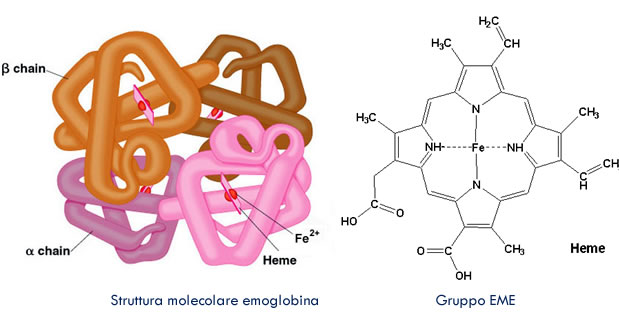
\includegraphics[width=\textwidth]{emoglobina-struttura.jpeg}
    \caption{Rappresentazione della struttura dell'emoglobina (a sinistra) e del gruppo 			 eme (a destra).}
    \label{fig:Structure}
\end{figure}
A livello polmonare, dove l'aria degli alveoli è a stretto contatto con le sottili pareti dei capillari sanguigni, le molecole di ossigeno passano nel sangue poiché la $P_{O_2}$ nell'aria alveolare è superiore alla $P_{O_2}$ del sangue. 
Di conseguenza l'ossigeno diffonde secondo il proprio gradiente di concentrazione dagli alveoli verso i capillari. 
Il passaggio si arresterà nel momento in cui la $P_{O_2}$ nel sangue che lascia i polmoni avrà eguagliato quella atmosferica negli alveoli. 
Quando il sangue arterioso raggiunge i capillari dei tessuti, il gradiente di concentrazione si inverte e l'ossigeno diffonde dal plasma alle cellule. 
La diffusione si arresta quando il sangue capillare venoso raggiunge la stessa pressione parziale di ossigeno dell'ambiente intracellulare circostante. 
La pressione parziale dell'aria alveolare può scendere qualora la ventilazione polmonare risulti inadeguata, o le pareti degli alveoli risultino per qualche ragione più spesse.


\subsection{Curva di dissociazione dell'emoglobina}

La relazione fisica tra la $P_{O_2}$ plasmatica e la quantità di ossigeno legata all'emoglobina è stata studiata in vitro((tipicamente tale studio viene effettuato a $pH$ 7.4 e ad una temperatura di $37^\circ$C) e viene rappresentata dalla caratteristica curva di dissociazione dell'emoglobina(Fig:\ref{fig:Dissociation Curve}). 
\begin{figure}[h!]
    \centering
    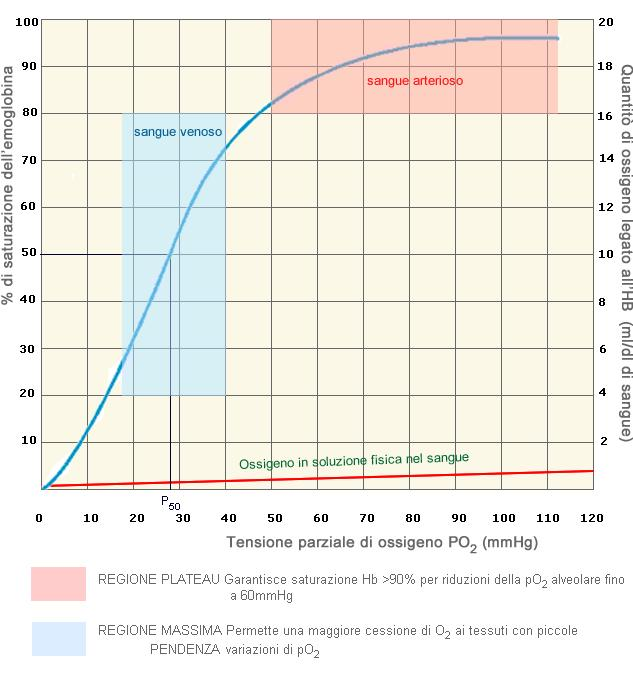
\includegraphics[width=\textwidth]{emoglobina2.jpeg}
    \caption{In figura è possibile osservare la percentuale di ossiemoglobina presente 					 sul totale dell'emoglobina in funzione della pressione parziale 							 dell'ossigeno $P_{O_2}$ in condizioni standard, ovvero ad un $pH$ 7.4 e ad 			 una temperatura di $37^\circ$C. 
			 L'area evidenziata in rosso corrisponde alla porzione di curva solitamente 			 relativa al sangue arterioso, in quanto più ossigenato, mentre la porzione 			 evidenziata in azzurro corrisponde al sangue venoso. 
			 Sul fondo è presente anche la retta che corrisponde all'ossigeno disciolto 			 direttamente nel plasma.}
    \label{fig:Dissociation Curve}
\end{figure}
In tale curva è presente un'ampia regione a bassa pendenza. 
Il fatto che tale regione risulti così ampia ed in prossimità del 100\% di saturazione fornisce un importante margine di sicurezza. 
Sebbene la $P_{O_2}$ a livello alveolare sia normalmente pari a 100 mm Hg, anche ad una pressione parziale di ossigeno intorno ai 70 mmHg (evenienza tipica di alcune malattie o della permanenza in alta quota) le percentuali di emoglobina saturata restino vicine al 100\%. 
\\Si analizzano ora alcuni importanti fenomeni in grado di influenzare la dissociazione dell'emoglobina. 
Il primo fra tutti è l'effetto Bohr, ossia l'effetto che hanno le variazioni delle concentrazioni di $H^+$ e $CO_2$ sul rilascio dell'ossigeno. 
Dove c'è più $CO_2$ disciolta in forma di Bicarbonato ($HCO_3^-$) l'emoglobina rilascia più facilmente Ossigeno e si carica di Anidride Carbonica (sempre in forma di Bicarbonato) (Fig:\ref{fig:CO2}). 
\begin{figure}[h!]
    \centering
    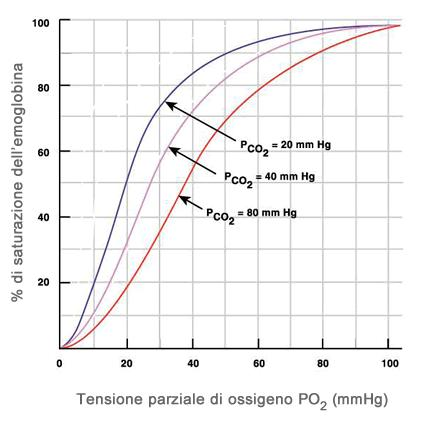
\includegraphics[width=\textwidth]{emoglobina-C02.jpeg}
    \caption{In figura è possibile notare la variazione dell'andamento della 	 		 			 dissociazione emoglobinica per varie pressioni parziali di $CO_2$ 							 ($P_CO_2$).}
    \label{fig:CO2}
\end{figure}
Lo stesso effetto si ottiene aumentando la concentrazione di ioni $H^+$, ossia abbassando il $pH$ e quindi acidificando il sangue: tanto più diminuisce il $pH$ ematico e tanto meno ossigeno rimane legato all'emoglobina. 
Non a caso, nel sangue l'anidride carbonica si trova disciolta prevalentemente in forma di acido carbonico ($H_2CO_3$), che si dissocia secondo la reazione:
\begin{equation*}
    \ce{CO_2 + H_2O <-> H_2CO_3 <-> H^+ + HCO_3^-}
\end{equation*}
Come anticipato, in ambiente acido l'emoglobina rilascia più facilmente l'ossigeno, mentre in ambiente basico il legame con l'ossigeno è più forte (Fig:\ref{fig:pH}).
\begin{figure}[h!]
    \centering
    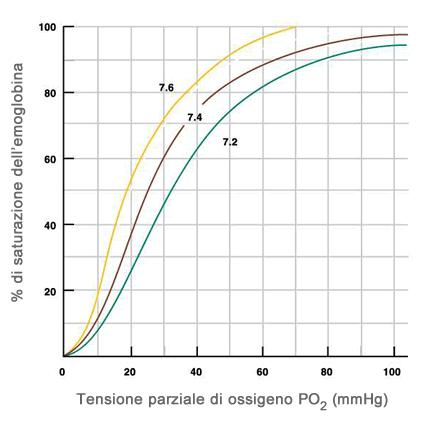
\includegraphics[width=\textwidth]{emoglobina-pH.jpeg}
    \caption{In figura è possibile notare la variazione dell'andamento della 							 dissociazione emoglobinica per diversi valori del $pH$ sanguigno.}
    \label{fig:pH}
\end{figure}
L'effetto Bohr risulta molto importante durante il lavoro muscolare intenso. 
Infatti nei tessuti maggiormente esposti allo sforzo si assiste ad un aumento locale della della pressione parziale di anidride carbonica, quindi dell'acidità ematica. 
Per quanto esposto, tutto ciò favorisce la cessione di ossigeno ai tessuti, spostando verso destra la curva di dissociazione dell'emoglobina.
\newline

Tra gli altri fattori in grado di modificare l'affinità dell'emoglobina per l'ossigeno vi è poi la temperatura (Fig:\ref{fig:T}). 
In particolare è stato misurato empiricamente che l'affinità dell'emoglobina per l'ossigeno diminuisce con l'aumento della temperatura corporea. 
Questo è particolarmente vantaggioso per ambienti freddi, dal momento che la temperatura del sangue polmonare (a contatto con l'aria dell'ambiente esterno) è minore di quella raggiunta a livello tessutale, dove la cessione di ossigeno risulta quindi facilitata.
\begin{figure}[h!]
    \centering
    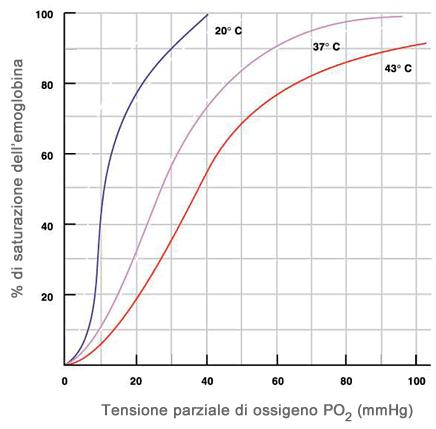
\includegraphics[width=\textwidth]{emoglobina-temperatura.jpeg}
    \caption{In figura è possibile notare la variazione dell'andamento della dissociazione emoglobinica per differenti valori di temperatura del sangue.}
    \label{fig:T}
\end{figure}
Un ulteriore agente in grado di modificare la curva di dissociazione dell'emoglobina è la presenza del 2,3 difosfoglicerato ($2,3-DPG$) (Fig:\ref{fig:DPG}). 
Tale molecola è un intermedio della glicolisi. 
Se le sue concentrazioni all'interno del globulo rosso aumentano, l'affinità dell'emoglobina per l'ossigeno diminuisce, facilitando quindi il rilascio di ossigeno ai tessuti. 
Non a caso, le concentrazioni di 2,3 difosfoglicerato all'interno dei globuli rossi aumentano, ad esempio, nelle anemie, nell'insufficienza cardio-polmonare e durante il soggiorno in altura. 
In generale, l'effetto del $2,3-DPG$ è relativamente lento, specie se paragonato alla rapida risposta alle variazioni di $pH$, temperatura e pressione parziale di anidride carbonica.
\begin{figure}[h!]
    \centering
    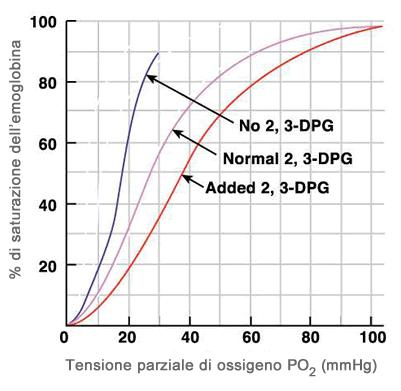
\includegraphics[width=\textwidth]{emoglobina-dpg.jpeg}
    \caption{In figura è possibile notare la variazione dell'andamento della 							 dissociazione emoglobinica per diverse concentrazioni di $2,3-DPG$ nel 					 sangue.}
    \label{fig:DPG}
\end{figure}

\newpage
\section{Il pulsossimetro}


\subsection{Principi alla base del funzionamento}

Il pulsossimetro ha contribuito ad innovare la medicina moderna, permettendo di monitorare in maniera non invasiva e continuativa la saturazione dell'emoglobina nel sangue arterioso. 
Il principio alla base del funzionamento di un pulsossimetro risiede nel diverso assorbimento, da parte di ossiemoglobina e desossiemoglobina, di certe lunghezze d'onda presenti nella regione del rosso e dell'infrarosso. 
Va considerato anche il fatto che le lunghezze d'onda prossime al giallo, al verde e al blu sono significativamente assorbite da alcuni tipi di tessuti e dall'acqua, perciò uno studio dell'andamento dell'assorbimento in tali regioni dello spettro elettromagnetico risulterebbe più complesso e meno preciso. 
L'ossiemoglobina risulta assorbire una maggiore quantità di luce nella regione dell'infrarosso ed una minore nella regione del rosso. 
Ciò è consistente con l'esperienza: il sangue ossigenato appare di un colore rosso acceso all'occhio umano, in quanto si ha un maggiore scattering della luce rossa, mentre il sangue meno ossigenato assorbe maggiormente la luce rossa e risulta pertanto più scuro. 
Il pulsossimetro emette pertanto due lunghezze d'onda a circa 660nm e 940nm da due diodi emettenti posti dallo stesso lato dello strumento. 
La luce attraversa la regione anatomica che si intende usare per la misurazione (solitamente una regione poco spessa e molto vascolarizzata come ad esempio la falange distale di un dito o il lobo di un orecchio) e viene rilevata da un fotodiodo posto dall'altra parte dello strumento di misura. 
La caratteristica del pulsossimetro di misurare solamente la saturazione dell'ossigeno del sangue arterioso è legata al ciclo cardiaco, dato che l'andamento della luce assorbita varia con il variare del volume del sangue. 
Il volume di sangue arterioso aumenta durante la sistole e diminuisce durante la diastole. 
Al confronto il volume sanguigno nelle vene e nei capillari resta praticamente costante se paragonato alle variazioni relative del volume di sangue arterioso, mentre ovviamente la pelle, le ossa ,il grasso ed altri tipi di tessuto mantengono praticamente invariato il loro volume. 
Pertanto si avrà una quantità minima costante di luce assorbita la quale darà un contributo costante di corrente (DC) in uscita dallo strumento, più una parte soggetta a pulsazioni dettate dal ritmo cardiaco, che sommerà un contributo variabile nel tempo di luce assorbita e dunque di corrente (AC). 
Il pulsossimetro calcola poi il rapporto di modulazione rosso/infrarosso, definito come:
\begin{equation}
    \label{eq:R}
    R=\frac{(A_{rosso,AC}/A_{rosso,DC})}{(A_{infrarosso,AC}/A_{infrarosso,DC})}
\end{equation}
dove $A$ denota l'assorbanza ed i pedici $AC$/$DC$ indicano le parti variabili/costanti del segnale in uscita dallo strumento. 
Si rammenta che l'assorbanza è definita come:
\begin{equation}
    \label{eq:Absorbance}
    A = -ln T = ln I_{0} - ln I_{1}
\end{equation}
dove $T$ è la trasmittanza e $I_{0}$ e $I_{1}$ sono le intensità della luce incidente e della luce che emerge dal campione attraversato ad una data lunghezza d'onda. 
\newline

A bassi livelli di saturazione dell'ossigeno, dove c'è una maggior quantità di desossiemoglobina, la variazione relativa di assorbanza dovuta alle pulsazioni cardiache è maggiore per la luce rossa rispetto a quella infrarossa ($A_{rosso,AC}>A_{infrarosso,AC}$). 
Si ha così un maggior valore di $R$. 
Una maggiore saturazione dell'ossigeno porterà invece la condizione $A_{rosso,AC}<A_{infrarosso,AC}$ da cui deriverà un minor valore di $R$. 
\newline

Il microprocessore di un pulsossimetro usa questo rapporto (calcolato su di una serie di pulsazioni diverse) per determinare l'$SpO_{2}$ basandosi su di una curva di calibrazione. 
Tale curva è generata empiricamente misurando $R$ in volontari sani la cui saturazione viene alterata in un range che va da circa il 70\% al 100\%. 
Per tale ragione misure di $SpO_{2}$ al di sotto del 70\% sono solitamente da considerarsi quantitativamente poco affidabili. 
Nonostante ciò risulta difficile pensare che una qualunque decisione medica potrebbe essere influenzata da questo fatto, dal momento che una $SpO_{2}$ al di sotto della suddetta soglia comporterebbe comunque un grave stato ipossico. 
Per capire come un pulsossimetro escluda l'influenza di tessuti, sangue venoso e capillare dal calcolo della $SpO_{2}$ consideriamo la legge di Lambert-Beer applicata al modello di un vaso sanguigno:
\begin{equation}
    \label{eq:Legge di Lambert-Beer}
    A = \varepsilon_{\lambda}lM
\end{equation}
dove $A$ è l'assorbanza, $\varepsilon_{\lambda}$ indica il coefficiente di assorbimento molare ad una lunghezza d'onda fissata ($\lambda$), $M$ è la molarità della soluzione ed $l$ è il cammino geometrico percorso dalla luce. 
In particolare  $\varepsilon_{\lambda}$ sarà una combinazione dei rispettivi coefficienti dell'ossiemoglobina e della desossiemoglobina, mentre $M$ sarà dato dalla concentrazione dell'emoglobina ed $l$ sarà il cammino geometrico percorso dalla luce all'interno del vaso sanguigno. 
A questo punto misurare semplicemente l'assorbanza offrirebbe una stima inesatta dell'$SpO_2$ arteriosa, dal momento che anche il sangue venoso offrirebbe un contributo al valore misurato. 
Per ovviare a questo problema un pulsossimetro misura le $variazioni$ di assorbanza nel tempo. 
\newline

L'assorbanza totale può essere scritta come somma dell'assorbanza arteriosa e dell'assorbanza venosa: 
\begin{equation*}
	A_T = A_A + A_V = \varepsilon_{\lambda,A}l_AM_A + \varepsilon_{\lambda,V}l_VM_V
\end{equation*}
derivando rispetto al tempo si ottiene:
\begin{equation*}
    \frac{d(A_T)}{dt} = \frac{d(\varepsilon_{\lambda,A}l_AM_A)}{dt} + 							\frac{d(\varepsilon_{\lambda,V}l_VM_V)}{dt} = \varepsilon_{\lambda,A}M_A					\frac{d(l_A)}{dt} + \varepsilon_{\lambda,V}M_V\frac{d(l_V)}{dt}
\end{equation*}
dove l'ultima uguaglianza vale dal momento che $\varepsilon_{\lambda}$ ed $M$ sono costanti una volta fissata la lunghezza d'onda e la specie chimica di emoglobina. 
Dal momento che, come già detto, la variazione di volume del sangue arterioso è considerevolmente maggiore di quella del sangue venoso si ha che:
\begin{equation*}
    \frac{d(l_A)}{dt} \gg \frac{d(l_V)}{dt}
\end{equation*}
dunque ha senso assumere $l_V$ circa costante ed approssimare così il secondo termine con 0. 
Perciò l'equazione finale diventa:
\begin{equation*}
    \frac{d(A_T)}{dt} = \varepsilon_{\lambda,A}M_A\frac{d(l_A)}{dt} = \frac{d(A_A)}				{dt}.
\end{equation*}
Ovviamente alla base di una buona misura vi è il fatto che la regione anatomica su cui si va ad eseguire l'acquisizione deve essere caratterizzata da una discreta perfusione sanguigna. 
In caso contrario verrebbe a mancare a condizione $\frac{d(l_A)}{dt} \gg \frac{d(l_V)}{dt}$ che permette di ignorare il contributo venoso, facendo risultare la misura molto meno affidabile.
\begin{figure}[h!]
    \centering
    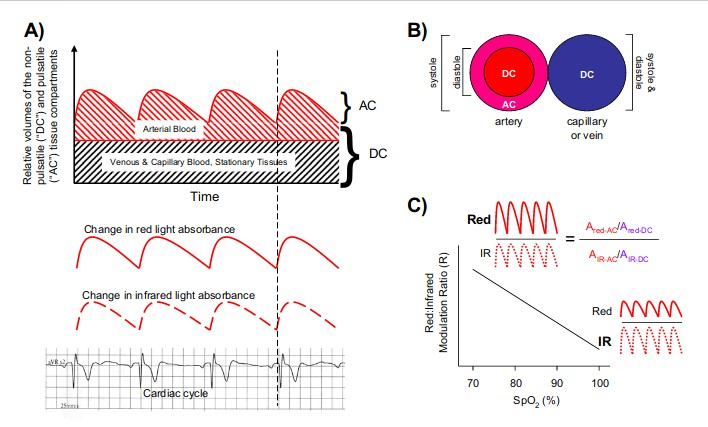
\includegraphics[width=\textwidth]{ACDC.jpg}
    \caption{In figura sono riportati vari aspetti fondamentali alla base della misura 					 di un pulsossimetro. 
   		     (A) Confronto tra l'andamento temporale dell'assorbimento luminoso 						 confrontato con ECG. 
 		     Si noti che il minimo dell'assorbimento si ha in prossimità dell'inizio 					 del complesso QRS nell'ECG. 
		     Si noti anche la presenza di una parte dell'assorbimento costante ed una 					 parte variabile dovuta esclusivamente al sangue arterioso. 
 		     (B) Confronto tra sezioni di arteria (sinistra) e vena (destra), atto ad 					 evidenziare come la variazione relativa di diametro sia considerevole solo 			 per il primo caso, che quindi risulterà essere l'unica causa della 						 componente variabile del segnale misurato. 
  		     (C) Esempio di retta di calibrazione standard utilizzata per convertire la 			 misura di $R$ in una misura dell'$SpO_2$. 
 		     Si osservi come un maggiore valore di $R$ implichi un minore valore di 					 $SpO_2$ e viceversa.}
    \label{fig:ACDC}
\end{figure}


\subsection{Vantaggi e svantaggi dei differenti tipi di pulsossimetro}

La ragione per cui le misurazioni dei pulsossimetri vengono prevalentemente effettuate su dita, naso, lobo dell'orecchio o fronte risiede nella maggiore vascolarizzazione della pelle in suddette regioni. 
I principali tipi di pulsossimetro utilizzati sono a clip (riutilizzabile) ed adesivi (usa e getta). 
I vantaggi dei pulsossimetri a clip sono: la rapidità di impiego, la comodità con cui possono essere impiegati per diverse zone del corpo in caso di pulsazioni di scarsa intensità (pinzando la regione si aumenta la pressione sanguigna e dunque anche l'intensità delle pulsazioni) ed il risparmio economico per alti numeri di prese dati da diversi pazienti, frutto della riutilizzabilità. 
I vantaggi dei pulsossimetri adesivi usa e getta risiedono nella minor trasmissione di infezioni nocosomiali, nel posizionamento più saldo e preciso in caso di pazienti in movimento (ad esempio durante visite sportive) e nella maggior precisione nel monitorare regioni acrali (queste sono maggiormente soggette a vasocostrizione e dunque presentano una difficoltà maggiore nelle misure pulsossimetriche). 
Ovviamente la zona sulla quale effettuare la misura ed il tipo di pulsossimetro più adatto saranno dettati dalle circostanze cliniche. 
Anche dopo aver scelto le opzioni ottimali si può incorrere in letture errate della misura a causa di diversi fattori, i quali verranno analizzati nella successiva sezione.

\begin{figure}[h!]
	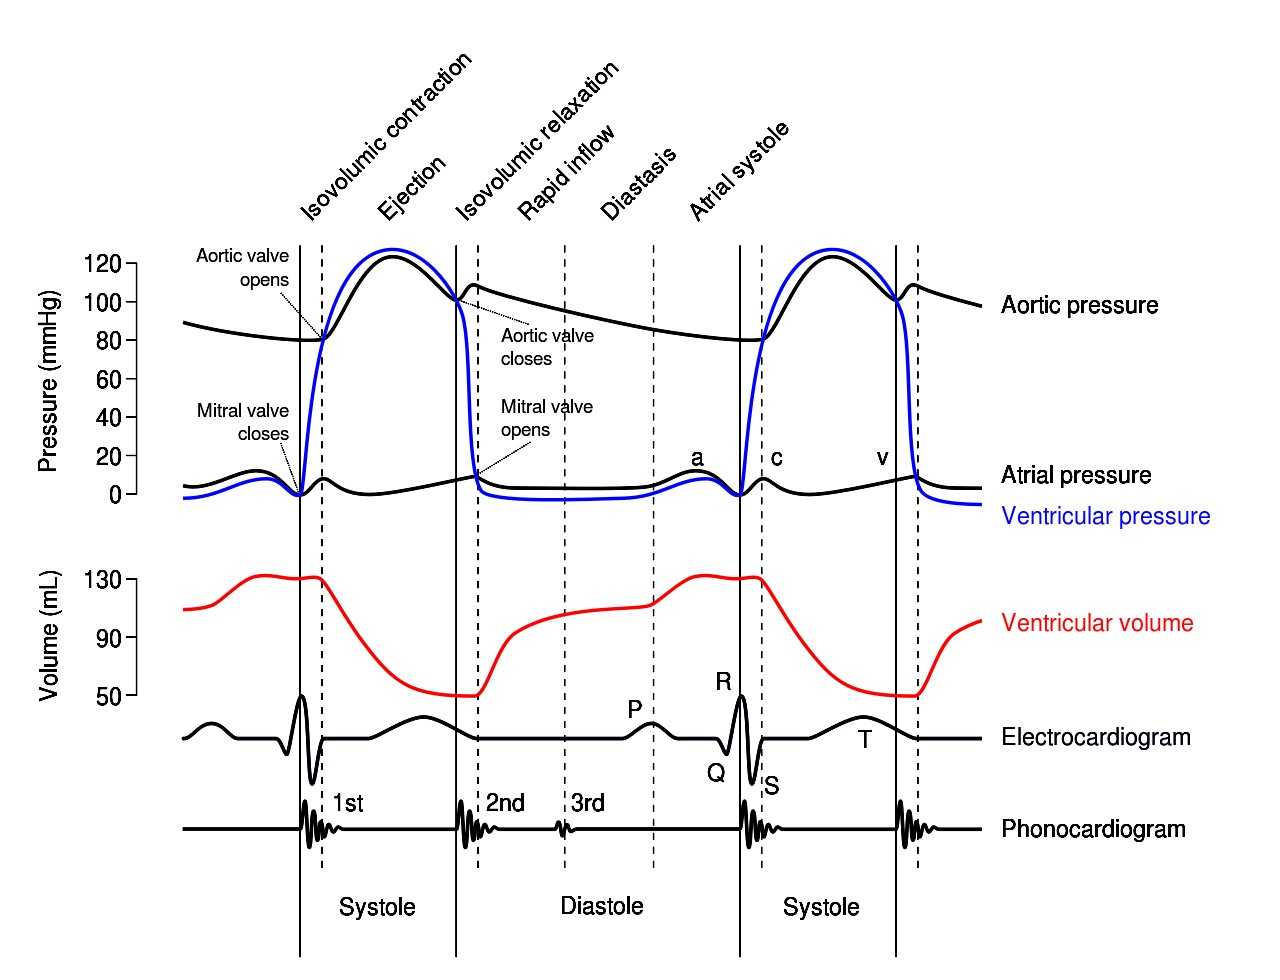
\includegraphics[width=\textwidth]{Wiggers_Diagram.jpg}
	\caption{In figura è possibile apprezzare l'andamento temporale di fonogramma, 					 	 elettrocardiogramma e diverse pressioni e volumi.
			 In particolare pressione in Aorta, pressione atriale, pressione 							 ventricolare e volume ventricolare.
			 La presenza in figura dell'elettrocardiogramma evidenzia la relazione tra 				 	 attività elettrica del cuore ed attività contrattile dei ventricoli.}
	\label{fig:Wiggers_Diagram}
\end{figure}


\subsection{Legame tra segnale pulsossimetrico ed ECG}

La grandezza fisica misurata dal pulsossimetro è la quantità di luce assorbita dai vari tessuti.
Ponendoci dunque in condizioni ideali, senza artefatti che compromettano la qualità della misura ed escludendo tutte le componenti costanti come ossa o cute, la principale variazione nel tempo è data dal sangue arterioso.
In particolare il parametro biologico misurato è il volume del sangue arterioso.
Da qui deriva il forte legame con l'elettrocardiogramma (ECG).
L'attività elettrica del cuore è ovviamente collegata all'attività contrattile che permette l'espulsione di sangue dall'organo stesso.
Come è possibile osservare in Fig:\ref{fig:Wiggers_Diagram} alla contrazione ventricolare corrisponde un aumento di pressione in Aorta dovuto all'aumento di flusso sanguigno.
Tale evento corrisponderà, dopo un certo intervallo temporale, ad un aumento del volume di sangue anche a livello periferico.
È proprio a causa di questa catena di ritardi temporali che in una misura pulsossimetrica non sarà possibile ricavare l'esatta posizione di un particolare evento cardiaco.
Ciò che risulta invece possibile ricavare è la distanza temporale tra un determinato evento e lo stesso nel ciclo successivo.
Riprendendo la Fig:\ref{fig:Wiggers_Diagram}, è evidente la difficoltà nel rilevare la posizione temporale del picco R misurando la pressione (o il volume) di un vaso sanguigno, non vi sono picchi o forme particolari che aiutino a riconoscerlo.
Se invece si considera la distanza temporale tra i due picchi R consecutivi (d'ora in avanti indicata con RR), tale distanza sarà la stessa fra qualsiasi altro punto ed il suo corrispondente nel ciclo cardiaco successivo.
Pertanto sarà possibile prendere un punto facilmente identificabile (nel caso del pulsossimetro il massimo del segnale, ovvero il minimo dell'assorbimento luminoso) e tramite la sua frequenza ricavare la frequenza cardiaca, o tramite il suo periodo ricavare l'RR, proseguendo l'analisi su tali misure senza più alcun tipo di errore sistematico.



\section{Fattori in grado di influenzare la misurazione}


\subsection{Differenza tra \texorpdfstring{$SpO_2$}{SpO_2} ed \texorpdfstring{$SaO_2$}{SaO_2}}

Per l'importanza che rivestirà in questa sezione va evidenziata la differenza che esiste tra una misura di $SaO_2$ ed una misura di $SpO_2$ (definiti dall'equazione $\ref{eq:definition}$).
La prima si effettua solitamente con ossimetri ed è la misura della saturazione dell'ossigeno nel sangue arterioso.
La seconda è la $SaO_2$ misurata da un pulsossimetro, ovvero la saturazione dell'ossigeno considerando solo l'emoglobina funzionale.
L'emoglobina funzionale è quella in grado di trasportare l'ossigeno, dunque parleremo solo di ossiemoglobina ($O_2Hb$) e desossiemoglobina (indicata con $HHb$ o semplicemente con $Hb$).
L'emoglobina non-funzionale consiste in quella non capace di trasportare ossigeno.
Quest'ultima è quasi esclusivamente rappresentata da emoglobina legata con qualcosa di diverso dall'ossigeno, come carbossiemoglobina ($COHb$), metaemoglobina ($MetHb$) o altre specie chimiche.
Pertanto le due misure sono ben diverse, anche se cercano di quantificare la stessa grandezza.
In particolare la misura reale dell'$SaO_2$ verrà sovrastimata dall'$SpO_2$ ogni volta che nel circolo sanguigno sarà presente dell'emoglobina non funzionale:
\begin{equation}
	\label{eq:definition}
	SpO_2 = \frac{[O_2Hb]}{[O_2Hb]+[HHb]}; \quad SaO_2 = \frac{[O_2Hb]}{[O_2Hb]+[HHb]+			[COHb]+[MetHb]+\ldots}
\end{equation}


\subsection{Cause di cali del rapporto segnale rumore}

L'ampiezza del segnale in uscita da un pulsossimetro riflette la modulazione luminosa indotta dalle pulsazioni cardiache. 
Come è possibile osservare in Fig:\ref{fig:ACDC} (A) il complesso QRS (visibile nell'elettrocardiogramma) induce un rapido aumento dell'ampiezza del segnale di un pulsossimetro. 
Segnali con scarsa ampiezza possono essere dovuti ad una riduzione della perfusione sanguigna. Tale condizione può avere varie cause: uso di vasocostrittori, ipotensione, shock ipovolemico, ipotermia o anomalie nel ritmo cardiaco. 
La riduzione dell'intensità delle pulsazioni nel sangue arterioso porta ad una diminuzione del rapporto segnale rumore del pulsossimetro ed eventualmente a letture instabili o eccessivamente basse della $SpO_2$


\subsection{Inquinamento da monossido di carbonio}

Il monossido di carbonio ($CO$) in condizioni standard è un gas incolore, inodore, insapore e non irritante. 
I pazienti vittime di avvelenamento da $CO$ possono presentare sintomi molto generici, come mal di testa e "sintomi simil-influenzali". 
Per le suddette ragioni è spesso difficile effettuare una rapida e chiara diagnosi. 
Il principale meccanismo patogenetico dell'avvelenamento da $CO$ è la sua enorme affinità con l'emoglobina (circa 240 volte quella dell'$O_2$) per formare Carbossiemoglobina ($COHb$), riducendo così la capacità dell'emoglobina di trasportare $O_2$ ed inducendo uno stato di ipossiemia nei tessuti. 
Il monossido di carbonio può anche danneggiare la mioglobina e le funzioni mitocondriali, aumentando l'attivazione della guanilato ciclasi che può indurre vasodilatazione e ipotensione. 
Ovviamente Il legame con l'emoglobina altera l'assorbanza misurata e conseguentemente il segnale in uscita dal momento che il fotodiodo standard di un pulsossimetro non riesce a distinguere le due molecole. 
La $COHb$ e la  $O_2Hb$ assorbono la luce rossa a 660nm in quantità molto simili e la $COHb$ assorbe una quantità estremamente bassa di luce infrarossa a 940nm. 
Riprendendo il fattore $R$ calcolato in precedenza ($\ref{eq:R}$), la $COHb$ ridurrà le concentrazioni di $Hb$ ed $O_2Hb$. 
In particolare l'assorbimento di luce rossa sarà ridotto, dato che $COHb$ e $O_2Hb$ hanno entrambe un assorbimento minore rispetto ad $Hb$ per quella data lunghezza d'onda, ed $R$ avrà un valore minore del previsto e conseguentemente l'$SpO_2$ verrà sovrastimata. 
Per distinguere le tre molecole sopracitate servirebbe un pulsossimetro in grado di lavorare con tre differenti lunghezze d'onda, e nonostante simili dispositivi esistano non risultano largamente impiegati.
\begin{figure}[h!]
    \centering
    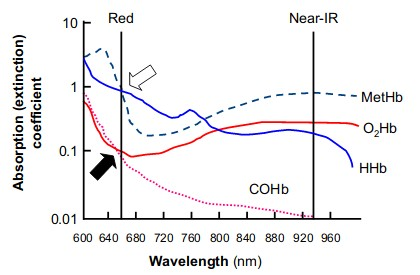
\includegraphics[width=\textwidth]{multidiss.jpg}
    \caption{In figura è possibile osservare l'andamento, in scala semilogaritmica, del 			 coefficiente di assorbimento per alcune specie di emoglobina al variare 					 della lunghezza d'onda della luce incidente. 
  		     Le due linee verticali indicano le lunghezze d'onda presso le quali lavora 			 un pulsossimetro standard. 
 		     Le due frecce vogliono far risaltare come la metaemoglobina ($MetHb$) e 					 l'emoglobina legata a monossido di carbonio ($COHb$) abbiano coefficienti 					 di assorbimento rispettivamente vicini a ossiemoglobina ($O_2Hb$) e 						 desossiemoglobina ($HHb$) in prossimità dei 660nm.} 
    \label{fig:multidissociation}
\end{figure}


\subsection{Anemia falciforme}

Spesso la presenza di questa malattia comporta crisi vaso-occlusive e sindrome acuta del torace, che a loro volta possono causare o essere peggiorate dall'ipossiemia; si ha così un circolo vizioso. 
La misurazione dell'$SpO_2$ effettuata con il pulsossimetro in pazienti affetti da anemia falciforme risulta ancora dibattuta. 
Uno studio su 17 pazienti malati ha mostrato nel calcolo dell'$SpO_2$ una sovrastima media del contenuto di $O_2Hb$ del 3.4\% ed una sottostima media della saturazione dell'1.1\%, nonostante queste osservazioni le letture dei pulsossimetri non hanno portato a formulare diagnosi di ipossiemie errate.% \cite{Sickle}. 
Altri studi suggeriscono che tali effetti si accentuino durante le crisi vaso-occlusive. 
Viene sottolineato come l'emoglobina degli eritrociti falciformi ($HbS$ dove S sta per sickle, ovvero falce in inglese), in condizioni normossiche (dove si ha scarsa polimerizzazione di $HbS$) abbia affinità con l'ossigeno simile a quella dell'emoglobina in pazienti sani, mentre in presenza di ipossiemia tale affinità cala, risultando in uno spostamento verso destra della curva di dissociazione emoglobinica classica. 
Dunque per qualsiasi pressione osmotica dell'ossigeno si avrà una minore $SpO_2$. Teoricamente questo effetto dovrebbe portare un maggior rilascio di ossigeno ai tessuti.


\subsection{Pulsazioni di origine venosa}

Le pulsazioni del sangue venoso possono contribuire a misurare livelli eccessivamente bassi di $SpO_2$, dal momento che nelle vene si ha minor presenza di $0_2Hb$ rispetto alle arterie. 
Questa complicazione può emergere nel caso di pulsossimetri adesivi eccessivamente stretti intorno al dito, gravi rigurgiti tricuspidali (reflusso di sangue attraverso la valvola tricuspide in concomitanza di una contrazione ventricolare destra), in caso di shock distributivo o qualora la posizione del paziente aumenti l'afflusso di sangue alla regione anatomica (ad esempio misurazioni effettuate sulla fronte di un paziente in posizione di Trendelenburg). 
In alcuni casi una parziale soluzione al problema può essere offerta dall'applicare una fascia elastica al pulsossimetro, la quale, se opportunamente regolata, eviterebbe l'eccessiva pressione che comporta la lettura delle pulsazioni venose.


\subsection{Movimenti eccessivi}

Sono state osservate misure di $SpO_2$ fino al di sotto del 50\% a seguito di tremori, convulsioni e movimenti in generale. 
Inoltre sono possibili, ma con minori probabilità, anche misure sovrastimate. 
A livello teorico, il movimento può indurre una variazione nella posizione dei tessuti rispetto al pulsossimetro lungo un dato arco temporale. 
Certe volte questa variazione può aumentare o "imitare" il segnale indotto dal cuore, dal momento che vene e tessuti si stanno ora muovendo, modulando così in maniera diversa la loro attenuazione luminosa. 
Comunque molti pulsossimetri moderni hanno algoritmi in grado di ridurre le false letture di $SpO_2$ causate dal movimento dei pazienti.


\subsection{Coloranti all'interno dei tessuti}

In medicina vengono impiegate varie sostanze coloranti. 
Ad esempio il blu di metilene viene utilizzato come agente riducente nella metaemoglobinemia. 
L'indigotina viene a volte impiegata per monitorare perdite di fluido amniotico o perdite del sistema urinario durante operazioni chirurgiche, dal momento che il sangue viene rapidamente ripulito da tale colorante. 
Il verde indocianina è invece impiegato in vari test diagnostici riguardanti il flusso sanguigno del fegato, funzioni epatiche ed angiografia oftalmica. 
Il picco di assorbimento luminoso del blu di metilene (Fig:\ref{fig:Coloranti}) è molto vicino all'assorbimento della desossiemoglobina nella regione adiacente. 
Il risultato è un maggior valore di $R$ con un conseguente valore minore di $SpO_2$.
\begin{figure}[h!]
    \centering
    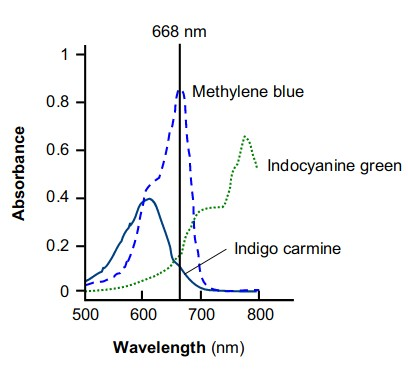
\includegraphics[width=\textwidth]{Coloranti.jpg}
    \caption{In figura è riportato l'andamento, in scala semilogaritmica, del 							 coefficiente di assorbimento al variare della lunghezza d'onda incidente 					 per tre coloranti di uso medico: blu di metilene, verde indocianina e 						 indigotina. 
    		 La linea verticale indica la lunghezza d'onda nei pressi del rosso che un 					 pulsossimetro standard prende in esame per effettuare le sua misure. 
    		 Si noti come il blu di metilene abbia un picco proprio nei pressi della 					 linea verticale.}
    \label{fig:Coloranti}
\end{figure}

In un campione di volontari con una $SpO_2 \geq$ 97\% si è osservato un drastico calo della stessa a seguito della somministrazione di blu di metilene (una soluzione di 5 ml con l'1\% di colorante), con un minimo del 65\%.% \cite{Pulseoximeter}. 
\newline

Il verde indocianina e l'indigotina invece non hanno un considerevole assorbimento luminoso nella regione dei 640 nm (Fig:\ref{fig:Coloranti}). 
Pertanto avranno un effetto minore sull'$SpO_2$ (per le stesse condizioni dello studio sopra esposto si nota una riduzione del $3\sim4$\% ). 
Il sunto di questa breve analisi è che l'utilizzo di coloranti comporta sempre una riduzione della $SpO_2$, tale riduzione dipende dall'assorbimento del colorante considerato nelle regioni in cui il pulsossimetro emette luce. 
Non vi è un metodo specifico per rimediare a questo tipo di errore, in quanto per grandi assorbimenti (come quello del blu di metilene) gli effetti dipendono anche dal paziente a causa di fattori come: pressione sanguigna, gittata cardiaca ed altri ancora.


\subsection{Forme ereditarie di emoglobina anormale}

Varianti piuttosto rare di emoglobina possono portare a misure erroneamente più basse della $SpO_2$. 
Ad oggi esistono oltre 1000 varianti di questa proteina e ne vengono scoperte continuamente di nuove. 
Esempi di alcune varianti che sono state osservate avere effetti sulla $SpO_2$ sono: $Hb$ Lensing, $Hb$ K\"oln, $Hb$ Hammersmith, $Hb$ Cheverly e $Hb$ Bonn. 
In uno studio eseguito su padre e figlia sono stati osservati valori del 10\% inferiori di $SpO_2$ causati dalla presenza di $Hb$ Lensing per circa l'11\% dell' emoglobina totale.% \cite{Pulseoximeter}.%wrong citing
Il fatto che l'affinità con l'ossigeno risulti normale suggerisce un'interferenza a livello di assorbanza da parte di questa variante dell'emoglobina. 
\newline

Uno altro studio effettuato su padre e figlio ha riportato risultati simili causati dall'$Hb$ Bonn.% \cite{Pulseoximeter}.%wrong citing 
In particolare quest'ultima variante presenta un picco di assorbimento a 668 nm (lo stesso del blu di metilene) e di conseguenza una maggiore assorbanza, un maggior valore di $R$ ed un minor valore di $SpO_2$. 
In altre parole l'$Hb$ Bonn si comporta in maniera simile alla desossiemoglobina o al blu di metilene. 
Effetti simili sono stati osservati anche per $Hb$ K\"oln ed $Hb$ Cheverly.


\subsection{Smalto per unghie}

Per coloranti esterni al corpo si ha una riduzione dell'$SpO_2$ proprio per gli stessi meccanismi visti nella sezione sui coloranti all'interno dei tessuti. 
Ovviamente il caso più frequente riguarda lo smalto per unghie durante misurazioni applicate alla falange distale, anche se moderni modelli di pulsossimetri sono in grado di attenuarne l'effetto. 
In particolare colori come il nero o il marrone hanno mostrato il maggior decremento medio, il quale però risultava comunque inferiore al 2\%.% \cite{Pulseoximeter}.%wrong citing


\subsection{Gravi anemie}

Teoricamente l'anemia non dovrebbe influenzare l'$SpO_2$, dal momento che l'emoglobina e la desossiemoglobina sono affette in maniera proporzionata. 
Ciò nonostante sono stati osservati rilevanti effetti da parte di gravi anemie sulla misura dell'$SpO_2$. 
Questo effetto viene ricondotto al fatto che la legge di Lambert-Beer ($\ref{eq:Legge di Lambert-Beer}$) non fornisce una spiegazione completamente corretta del fenomeno nel mondo reale, in quanto il cammino ottico della luce viene assunto come unico e ben definito. 
Al contrario nella realtà la luce è soggetta a scattering ogni volta che incontra un eritrocita e pertanto il cammino dipende dal numero di globuli rossi incontrati. 
Dunque ci si aspetterebbe un minor valore di $SpO_2$ in soggetti anemici, dal momento che i pulsossimetri vengono calibrati su soggetti sani, ovvero con un maggior numero di eritrociti. 
Generalizzando il discorso, in pazienti con un ematocrito considerevolmente inferiore alla norma, l'$SpO_2$ sottostima la misura reale dell'$SaO_2$. 
Va sottolineato che la sottostima dovuta ad anemia è lieve in condizioni normossiche, mentre si aggrava notevolmente in condizioni di ipossiemia.


\subsection{Metaemoglobinemia}

La metaemoglobina ($MetHb$) si ottiene quando l'atomo di $Fe$ del gruppo eme si ossida, passando dallo stato ferroso ($Fe^{+2}$) allo stato ferrico ($Fe^{+3}$). 
La $MetHb$ compromette il trasporto di ossigeno ai tessuti tramite due effetti: (i) la molecola stessa ha una minore affinità con l'ossigeno, (ii) la $MetHb$ causa uno spostamento della curva di dissociazione dell'emoglobina normale (Fig:\ref{fig:Dissociation Curve} ) verso sinistra, riducendo la quantità di ossigeno rilasciato ai tessuti a parità di pressione parziale dell'$O_2$. 
La maggior parte dei pazienti affetti da eccessivi livelli di $MetHb$ deriva dall'assunzione di agenti chimici ossidanti, come: nitriti, nitrati, coloranti all'anilina, derivati dell'anilina (ad esempio Dapsone e fenacetina), sulfamidici o lidocaina. 
Basta una concentrazione di 1.5 g/dL di $MetHb$ (circa il 10\%-20\% del totale dell'$Hb$) per causare cianosi, anche se questo effetto è meno evidente in pazienti anemici a causa del minore livello assoluto di $MetHb$. 
Valori dal 20\% al 45\% possono portare a debolezza, emicranie e mancanza di fiato, mentre valori oltre il 50\% possono essere letali. 
La $MetHb$ assorbe molta più luce infrarossa di emoglobina e desossiemoglobina, mentre il suo assorbimento della luce rossa è molto simile a quello della desossiemoglobina (Fig:\ref{fig:multidissociation}). 
Dunque la metaemoglobina assorbe in grandi quantità sia luce rossa che infrarossa, pertanto il valore di $R$ sarà più prossimo ad 1, risultando in una stima dell'$SpO_2$ compresa tra l'80\% e l'85\%. 
Dunque questo tipo di problema è diverso dai precedenti incontrati. 
Non è più possibile correggere l'errore sull'$SpO_2$  dal momento che non è noto se si stia sottostimando o sovrastimando (in caso di gravi ipossiemie l'$SpO_2$ può risultare $\leq$ 85\%) la reale misura. 
Persino le soluzioni in grado di bloccare momentaneamente il problema non appaiono semplici da trattare. 
Il principale agente riducente impiegato per la metaemoglobinemia è il blu di metilene, che come già detto comporta ulteriori problemi sulla misura dell'$SpO_2$.


\subsection{Sulfoemoglobinemia}

La Sulfoemoglobina ($SulfHb$) si forma in maniera simile alla metaemoglobina, con la differenza che, oltre all'atomo di $Fe^{+3}$, l'anello porifirinico del gruppo eme contiene ora anche un atomo di zolfo. 
Solamente una concentrazione di 0.5 g/dL di tale molecola può portare cianosi. 
Il legame con lo zolfo è irreversibile e la peggior conseguenza è l'impossibilità da parte della molecola di $SulfHb$ di trasportare ossigeno. 
La presenza di $SulfHb$ chiaramente riduce il trasporto di ossigeno, ma sposta anche la curva di dissociazione dell'emoglobina (Fig:\ref{fig:Dissociation Curve}) verso sinistra, facilitando il rilascio dell'ossigeno ai tessuti (contrariamente a quanto avveniva per la presenza di $MetHb$). 
Dunque a parità di concentrazioni la $SulfHb$ porta meno complicazioni mediche rispetta alla $MetHb$, ciò nonostante elevate concentrazioni di sulfoemoglobina possono danneggiare irreparabilmente il trasporto di ossigeno riducendo l'ossiemoglobina.


\subsection{Posizionamento dello strumento e luce ambientale}

Se il pulsossimetro viene posizionato in una regione non adatta, perché poco vascolarizzata o eccessivamente spessa, l'eccessivo assorbimento della luce da parte dei tessuti incontrati porta ad avere un valore di $R$ prossimo ad 1, con conseguenze simili a quelle esposte nel paragrafo sulla metaemoglobinemia. 
La radiazione ambientale invece svolge l'effetto opposto, ma portando spesso la stessa conseguenza. 
Un eccessiva radiazione ambientale può far saturare il livello di luce assorbita per entrambe le lunghezze d'onda, portando così nuovamente il valore di $R$ in prossimità di 1. 
Questo secondo tipo di problema viene ovviato dai pulsossimetri più moderni, che risultano in grado di sottrarre la radiazione proveniente dall'ambiente alla radiazione assorbita. 
Per una migliore precauzione è comunque consigliabile eseguire la misurazione in luoghi non eccessivamente luminosi o schermare lo strumento con un materiale opaco.


\subsection{Sepsi e shock settico}

Allo stato attuale vi sono risultati differenti su come sepsi e shock settico possano influenzare la misura dell' $SpO_2$. 
In uno studio eseguito su 80 pazienti la presenza di suddette patologie ha comportato una $SpO_2$ che sottostimava dell'1.4\% la reale saturazione.% \cite{Pulseoximeter}. 
Sebbene tale modifica sia importante, sarebbe raramente in grado di influenzare una diagnosi. 
Un'ipotesi avanzata per spiegare questo fenomeno è la seguente: la vasodilatazione indotta da sepsi porta alla formazione di shunt artero-venosi, con la conseguente rilevazione di alcune pulsazioni venose come se fossero arteriose. 
Di contro, uno studio su 88 pazienti gravemente affetti da sepsi ha evidenziato una notevole sovrastima della saturazione da parte dell'$SpO_2$ (del valore di circa il 5\%) nei casi di ipossiemia (ovvero per $SpO_2 \leq 90\%$). 
Va comunque fatto notare che molti studi arrivano a risultati largamente differenti ed alle volte contraddittori. 
Probabilmente tali risultati possono essere letti così: i diversi effetti delle sepsi e le sue innumerevoli tipologie risultano difficilmente trattabili come un unico agente che modifichi in maniera uniforme le letture di $SpO_2$, e pertanto serve una maggiore catalogazione in "sotto-categorie" per ottenere risultati più concordi.




\chapter{Processing di serie temporali pulsossimetriche}


\subsection{Introduzione}

In questo capitolo saranno esposti gli strumenti matematici utilizzati per analizzare segnali pulsossimetrici.
Di ogni strumento verranno prima date definizione, proprietà ed utilizzi comuni.
In seguito verrà esposta la struttura del processing dei segnali, mostrando come ogni strumento viene impiegato all'interno del caso specifico ed il risultato a cui si arriva.
Infine verrà esposta la struttura del codice relativo all'estrazione delle features, mostrando in base a che criterio sono selezionate e come sia possibile ricavarle dal segnale processato, arrivando così a realizzare un database di features molto pratico per la successiva analisi.


\section{Strumenti matematici}


\subsection{Il filtro di Butterworth}

Un filtro viene definito come un processo o un dispositivo in grado di rimuovere caratteristiche indesiderate da un segnale.
Il filtro di Butterworth è un tipo di filtro che agisce sulle frequenze che compongono il segnale ed è realizzato per avere la risposta in frequenza più piatta possibile.
Il suo impiego è dunque adatto ai casi in cui si desidera avere il minor effetto possibile sulle frequenze della banda passante.
Introduciamo brevemente il concetto di \textit{polinomio di Butterworth} per descrivere in seguito la funzione di trasferimento di tale filtro.
Viene definito \textit{polinomio di Butterworth di ordine n} $(\beta^{(n)}(s) )$ un polinomio a coefficienti reali avente le seguenti caratteristiche:\begin{itemize}
    \item gli zeri del polinomio devono giacere sulla circonferenza di raggio unitario 				  e centrata nell'origine del piano complesso;
    \item se n è dispari le radici devono essere le 2n-esime radici di 1 a parte reale 				  negativa;
    \item se n è pari le radici devono essere le 2n-esime radici di -1 a parte reale 				  negativa;
\end{itemize}
il raggio della circonferenza diventerà $\omega_0$ quando il polinomio sarà espresso nella forma $\beta^{(n)}(\frac{s}{\omega_0})$.
\begin{table}[h]
    \begin{tabular}{
        S[table-format = 4]
        S[table-format = 12]}
        \toprule
    {Ordine} & {Polinomio di Butterworth}\\
    \midrule
    {0}  &  {$1$} \\
    {1}  &  {$s+1$} \\
    {2}  &  {$s^2+\sqrt{2}s+1$} \\ 
    {3}  &  {$s^3+2s^2+2s+1$} \\ 
    \bottomrule
\end{tabular}
\caption{\it{Tabella contenente i primi 4 polinomi di Butterworth normalizzati (ovvero 					 con $\omega_0=1$).}}
\end{table}
\newline

La funzione di trasferimento di un filtro di Butterworth è definita come il rapporto tra due polinomi di Butterworth, dove spesso a livello pratico al numeratore si usa il polinomio di ordine 0.
Il modulo di tale funzione risulta esprimibile come:
\begin{equation}
	|H(j\omega)| = \frac{1}{\sqrt{1+(\omega / \omega_0)^{2n}}}
\end{equation}
dove $j$ è l'unità immaginaria, e ci si avvale del cambio di variabile $s = j\omega$.
Ora risulta possibile capire perché tale filtro risulti massimamente piatto, in quanto le derivate della funzione di trasferimento calcolate in $\omega = 0$ sono nulle sino all'ordine $n$. 



\subsection{Media mobile}

La media mobile è uno strumento statistico molto utilizzato nell'analisi dati.
In breve consiste nel calcolare la media di un sottoinsieme compatto di dimensioni fissate, dopodiché si variano gli elementi del sottoinsieme e si ripete l'operazione.
Considerando una serie temporale {$y_t$} con $t = 1,2,\ldots,T$ per la variabile y, la media mobile al tempo $t$ è definita come:
\begin{equation}
	mm_t = \frac{1}{m_1+m_2+1} \displaystyle \sum_{i=-m_1}^{m_2} k_iy_{t+i} 
\end{equation}
dove $m_1$ corrisponde al numero di elementi precedenti ad $y_t$ che si desidera cosiderare, $m_2$ corrisponde analogamente agli elementi successivi e $k_i$ corrisponde all'i-esimo peso della media mobile.
Si noti come $m_1+m_2+1$ corrisponda alla dimensione del sottoinsieme di cui si intende calcolare la media.
Si parlerà di media mobile $centrata$ qualora $m_1=m_2$, $semplice$ se $k_i=1 \quad \forall i$ e $simmetrica$ nel caso in cui sia $centrata$ e valga $k_i=k_{m-i} \quad \forall i \in [-m, 0]$ dove $m=m_1=m_2$.
L'utilizzo della media mobile sulle serie temporali è spesso legato al voler ottenere un segnale più liscio rispetto a quello di partenza.
Tale effetto è la conseguenza del minor peso dato ad eventi di durata $\Delta t < m_1+m_2+1$ rispetto al peso che viene dato ad eventi di durata maggiore o uguale al periodo della finestra.
Dunque la media mobile può attenuare gli effetti a breve termine e far risaltare così gli effetti a lungo termine.
Per la stessa ragione la media mobile può essere considerata come un filtro passa-basso, in quanto attenua gli effetti dei periodi minori (alte frequenze).
Esistono vari altri tipi di media mobile come quella cumulativa, quella esponenziale o quella modificata, ma tali tipi non verranno approfonditi in quanto l'unica media mobile utilizzata di seguito sarà una media mobile semplice e simmetrica.


\subsection{Trasformata di Fourier, trasformata di Hilbert e Fast Fourier Transform}

La trasformata di Fourier è uno degli strumenti più utilizzati in assoluto nell'ambito dell'analisi dei segnali.
La sua utilità risiede nella possibilità di scomporre un segnale in onde sinusoidali di diverse ampiezze e frequenze, le quali sommate ci restituiscono il segnale di partenza.
Si può passare così dal dominio del tempo (dove avremo valori della grandezza misurata in funzione del tempo) al dominio delle frequenze (dove avremo valori di ampiezza in funzione della frequenza), ottenendo così una diversa espressione dello stesso segnale, la quale facilita certi tipi di analisi e l'implementazione di certe operazioni (come la differenziazione o la convoluzione).
La definizione matematica è la seguente:
\begin{equation}
	\label{eq:Fourier}
	\mathcal{F}(f) = \int_{-\infty}^{+\infty}x(t)e^{2 \pi i f t} dt
\end{equation}
dove $\mathcal{F}(f)$ indica la trasformata di Fourier di $x(t)$.
Analogamente è possibile definire l'antitrasformata di Fourier $\mathcal{F}^{-1}(x)$ come:
\begin{equation}
	\mathcal{F}^{-1}(t) = \int_{-\infty}^{+\infty}y(f)e^{-2 \pi i f t} df
\end{equation}
Queste particolari trasformazioni godono di diverse proprietà\footnote{Dove è stato assunto che $F(t),G(t)$ ed $H(t)$ siano funzioni integrabili e si indicano per brevità le trasformate di Fourier con $\hat{F}(f), \hat{G}(f)$ ed $\hat{H}(f)$ }:
\begin{itemize}
	\item[1)] se $H(t)=\alpha F(t)+\beta G(t)$ allora $\hat{H}(f) = \alpha \hat{F}(f)+					  \beta \hat{G}(f) \quad \forall \alpha,\beta \in \mathbb{C}$;
	\item[2)] se $H(t)=F(t-t_0)$ allora $\hat{H}(f) = e^{-2\pi ift_0}\hat{F}(f) \quad 					  \forall t_0 \in \mathbb{R}$; 
	\item[3)] se $H(t)=e^{2\pi if_0t}F(t)$ allora $\hat{H}(f) = \hat{F}(f-f_0) \quad 					  \forall f_0 \in \mathbb{R}$;
	\item[4)] se $H(t) = F(\alpha t)$ allora $\hat{H}(f) = \frac{1}{|\alpha|} \hat{F}					  (f/\alpha) \quad \forall \alpha \in \mathbb{R}-{0}$;
	\item[5)] se $H(t) = \overline{F(t)}$ allora $\hat{H}(f) = \overline{ \hat{F} (-f)}					  $;
	\item[6)] se $H(t)=\frac{dF(t)}{dt}$ allora $\hat{H}(f) = 2\pi if\hat{F}(f)$
	\item[7)] se $H(t)=(F*G)(t)$ allora $\hat{H}(f) = \hat{F}(f) \cdot \hat{G}(f)$;
	\item[8)] se $H(t)$ è inoltre continua ed $\hat{H}(f)$ è integrabile allora $						  \mathcal{F}^2 = H(-t)$, $\mathcal{F}^3 = \mathcal{F}^{-1} $ e $							  \mathcal{F}^4 = H(t)$ dove $\mathcal{F}^n$ indica la trasformata di 						  Fourier eseguita $n$ volte e con $n=-1$ si indica l'antitrasformata;	
\end{itemize}
La prima proprietà è ovviamente la linearità, la seconda e la terza prendono il nome di shifting temporale e shifting di frequenza, mentre la quarta è la riscalabilità temporale.
Si noti come porre $\alpha = -1$ nella quarta ci dia un'inversione temporale.
Si noti infine come la sesta e la settima proprietà permettono di comrendere come la trasformata di Fourier semplifichi l'implementazione di derivata e convoluzione, qualità accennata in precedenza.
\newline

Un limite applicativo della definizione $\ref{eq:Fourier}$ consiste nella scomoda presenza di una somma infinita di termini infinitesimi.
Tale richiesta comporta una conoscenza continua della funzione da trasformare ed un infinito tempo per computare la trasformazione.
Perciò nella pratica la trasformata di Fourier dovrà essere approssimata da qualcosa di computabile, quel qualcosa è la trasformata di Fourier discreta o DFT.
La trasformata di Fourier discreta (DFT) è definita dalla formula:
\begin{equation}
	\label{eq:DFT}
	X_k=\sum_{n=0}^{N-1} x_ne^{\frac{2 \pi i}{N} nk}
\end{equation}
Dove $k$ è un numero intero che va da 0 a $N-1$ e dove $x_n$ è la successione dei valori della nostra serie.
Si noti che non vi è alcun concetto di tempo nella definizione di DFT, la quale può quindi essere applicata solo a serie con punti equispaziati nel tempo, onde evitare risultati totalmente errati.
La DFT permette di computare una trasformata di Fourier approssimata, ma richiede un dispendio di tempo enorme per grandi moli di dati, portando non pochi problemi dal punto di vista pratico.
Quest'ultimo ostacolo venne superato grazie alla Fast Fourier Transform (FFT).
Anche per la FFT esistono diverse forme per implementare l'algoritmo, ma in generale il punto comune a tutte è la divisione del problema in vari sub-problemi di difficoltà triviale, computando poi il risultato finale a partire da questi risultati parziali.
Tale principio prende il nome di \textit{Divide et impera}.
È importante sottolineare un'ultima volta la differenza tra FFT, DFT e Fourier Transform.
La DFT \underline{approssima} il risultato della Fourier transform, la quale richiederebbe infinite informazioni, infinita precisione ed infinito tempo per essere computata realmente.
La FFT \underline{riduce il tempo di computazione} della DFT, ma mantiene la stessa precisione nel risultato ottenuto.
Dunque il passaggio dalla trasformata di Fourier alla DFT è dettato dai limiti di realizzazione pratica e comporta una perdita di precisione, mentre il passaggio dalla DFT alla FFT è dettato dal notevole risparmio di tempo che comporta e non incide sulla precisione. 
Verrà analizzato ora l'algoritmo impiegato all'interno del codice: la Radix-2 Decimation-In-Time (Radix-2 DIT).
La radix-2 DIT è l’esempio più semplice e comune dell'algoritmo di Cooley-Tukey per computare una FFT, anche se le implementazioni altamente ottimizzate di tale algoritmo utilizzano altre forme.
La Radix-2 DIT divide una DFT di dimensione $N$ in due DFT di dimensione $N/2$ ad ogni ricorsione (da qui il nome “ Radix-2”).
Ricordando che la DFT è definita da \ref{eq:DFT}, la Radix-2 DIT prima computa le DFT degli input di indice pari ($x_{2m}=x_0 , x_2 ,\ldots , x_{N-1}$) e degli input di indice dispari ($x_{2m+1}= x_1 , x_3 ,\ldots , x_{N-1}$) separatamente, e poi combina i due risultati per ottenere la DFT di tutta la sequenza.
Questa idea può essere poi utilizzata ricorsivamente per ridurre il tempo di esecuzione complessivo a $O(N log N)$.
Questa forma semplificata presuppone che $N$ sia una potenza di 2; dal momento che è quasi sempre possibile "attaccare" degli zeri alla fine della serie, spesso non è una restrizione importante.
Come detto la Radix-2 DIT riarrangia la DFT della funzione $x_n$ in due parti: una somma su tutti i numeri di indice pari $n=2m$ e una somma su tutti i numeri di indice dispari $n=2m+1$:
\begin{equation}
	X_k=\sum_{m=0}^{N/2-1} x_{2m} e^{-\frac{2\pi i}{N} (2m)k} + \sum_{m=0}^{N/2-1} 				x_{2m+1} e^{-\frac{2 \pi i}{N} (2m+1)k}
\end{equation}
È quindi chiaro che le due somme sono le DFT della parte ad indici pari $x_{2m}$ e la DFT della parte ad indici dispari $x_{2m+1}$ della funzione $x_n$.
Indichiamo la DFT degli input con indice pari $x_{2m}$ con $E_k$ e la DFT degli input con indice dispari $x_{2m+1}$ con $O_k$ e otteniamo:
\begin{equation}
	X_k=\underbrace{\sum_{m=0}^{N/2-1} x_{2m} e^{-\frac{2 \pi i}{N/2}mk}}_{DFT\; della			\; parte\; ad\; indici\; pari\; di\; x_n} + e^{-\frac{2 \pi i}{N}k} 						\underbrace{\sum_{m=0}^{N/2-1} x_{2m+1}e^{-\frac{2 \pi i}{N/2}mk}}_{DFT\; della\; 			parte\; ad\; indici\; dispari\; di\; x_n} = E_k + e^{-\frac{2 \pi i}{N}k} O_k .
\end{equation}
Grazie alla periodicità dell’esponenziale complesso, $X_{k+\frac{N}{2}}$ si può anche ottenere a partire da $E_k$ ed $O_k$
\begin{align}
	X_{k+\frac{N}{2}} &= \sum_{m=0}^{N/2-1} x_{2m} e^{-\frac{2 \pi i}{N/2}m(k+\frac{N}			{2})} + e^{-\frac{2 \pi i}{N}(k+\frac{N}{2})} \sum_{m=0}^{N/2-1}  x_{2m+1} e^{-				\frac{2 \pi i}{N/2}m(k+\frac{N}{2})} \\
	&=\sum_{m=0}^{N/2-1} x_{2m} e^{-\frac{2 \pi i}{N/2}mk} e^{-2 \pi mi} + e^{-\frac{2 			\pi i}{N}k} e^{-\pi i} \sum_{m=0}^{N/2-1} x_{2m+1} e^{-\frac{2\pi i}{N/2} mk} e^{-2 	\pi mi} \\
	&=\sum_{m=0}^{N/2-1} x_{2m} e^{-\frac{2 \pi i}{N/2}mk} - e^{-\frac{2 \pi i}{N}k} 			\sum_{m=0}^{N/2-1} x_{2m+1} e^{-\frac{2\pi i}{N/2} mk} \\
	&=E_k - e^{-\frac{2 \pi i}{N}k} O_k
\end{align}
dove $X_k$ può essere riscritto come:
\begin{align}
	X_k = E_k+ e^{-\frac{2 \pi i}{N}k}O_k \\
	X_{k+\frac{N}{2}} = E_k -e^{-\frac{2 \pi i}{N}k}O_k
\end{align}
Questo risultato, che esprime ricorsivamente la DFT di lunghezza $N$ in termini di due DFT di dimensione $N/2$, è il nucleo della Radix-2 DIT FFT. L’algoritmo deve la sua velocità al fatto che riutilizza i risultati delle computazioni intermedie per calcolare gli output delle DFT.
Da notare che gli output finali sono ottenuti da una combinazione di $E_k$ e $O_k$ $exp(-2 \pi i /N)$ che è semplicemente una DFT di dimensione 2; quando questo viene generalizzato a radici più grandi, la DFT di dimensione 2 è sostituita da una DFT maggiore.
Questo processo è un esempio di algoritmo “$divide$ $et$ $impera$”.
In ultimo la trasformata di Hilbert di un segnale $u(t)$ viene definita come:
\begin{equation}
	\mathcal{H}(u(t)) = - \frac{1}{\pi} \lim_{\epsilon \to 0}\int_{\epsilon}^{+\infty} 			\frac{u(t+\tau)-u(t-\tau)}{\tau} d\tau
\end{equation}
e può essere interpretata come il valore principale della convoluzione con il kernel di Cauchy ($1/\pi t$), in quanto l'integrale di convoluzione con tale kernel non sempre converge.
La traformata di Hilbert serve per la computazione del segnale analitico ed è collegata alla trasformata di Fourier dalla seguente relazione:
\begin{equation}
	\mathcal{H}(u(t)) = \mathcal{F}^{-1}(\;(-i \cdot sgn(t)) \cdot \mathcal{F}(u(t))\;) 
\end{equation}
dove $sgn(t)$ è la funzione segno e vale 0 per $t=0$, $t/|t|$ altrimenti.



\subsection{Inviluppo, segnale analitico e demodulazione}

L'inviluppo superiore di un'onda può essere pensato come l'ampiezza massima istante per istante assunta dall'onda.
L'inviluppo inferiore è l'analogo per l'ampiezza minima.
Risulta quindi intuitivo come queste due curve racchiudano sempre l'onda e siano tangenti, la prima a tutti i picchi, le seconda a tutti i ventri.
Le operazioni di demodulazione si avvalgono di tale concetto per eliminare l'inviluppo delle curve (o meglio, renderlo piatto), in modo da avere tutti i picchi alla stessa altezza e tutti i ventri alla stessa altezza.
\newline
Un segnale analitico è una funzione complessa che non ha componenti a frequenza negativa.
Le parti reali e immaginarie di un segnale analitico sono funzioni reali collegate tra di loro dalla trasformata di Hilbert.
Questa rappresentazione facilita molte operazioni matematiche.
L’idea di base è che le componenti a frequenza negativa della trasformata di Fourier di una funzione reale siano superflue, grazie alla simmetria di Hermitiana di tale spettro.
Se $s(t)$ è una funzione a valori reali avente trasformata di Fourier $S(f)$, allora la trasformata ha simmetria Hermitiana lungo l’asse $f=0$:
$S(-f)=S(f)^*$, dove $S(f)^*$ è il complesso coniugato di $S(f)$. La funzione:
\begin{align}
	S_a(f) &:= \begin{cases} 2S(f) & f>0 \\ S(f) & f=0 \\ 0 & f<0 \end{cases} \\
	&= \underbrace{2u(f)}_{1+sgn(f)}S(f) = S(f)+sgn(f)S(f)
\end{align}
Dove:
\begin{itemize}
	\item $u(f)$ è la funzione a gradino di Heaviside
	\item $sgn(f)$ è la funzione segno
\end{itemize}
Contiene solo componenti di frequenza non negative di $S(f)$ e l’operazione è reversibile, grazie alla simmetria Hermitiana di $S(f)$:
\begin{align}
	S(f) &= \begin{cases} \frac{1}{2} S_a (f), & f>0 \\ S_a(f), & f=0 \\ \frac{1}{2}			S_a(-f)^* & f<0 \end{cases} \\
	&=\frac{1}{2}[S_a(f)+S_a(-f)^*].
\end{align}
Il segnale analitico di $s(t)$
È la trasformata di Fourier inversa di $S_a(f)$:
\begin{align}
	S_a(t)&:= \mathcal{F}^{-1}[S_a(f)] \\
	&= \mathcal{F}^{-1}[S(f)+sgn(f) \cdot S(f)] \\
	&=\underbrace{\mathcal{F}^{-1}[S(f)]}_{s(t)} + \overbrace{ \underbrace{\mathcal{F}			^{-1} [sgn(f)]}_{j\frac{1}{\pi t}} * \underbrace{\mathcal{F}^{-1}[S(f)]}_{s(t)} }			^{convoluzione} \\
	&=s(t)+j \underbrace{[\frac{1}{\pi t}*s(t)]}_{\mathcal{H}[s(t)]} \\
	&=s(t) + j\hat{s}(t)
\end{align}
Dove
\begin{itemize}
	\item $\hat{s}(t):=\mathcal{H}[s(t)]$ è la trasformata di Hilbert di $s(t)$.
	\item $*$ è il simbolo della convoluzione.
	\item $j$ è l’unità immaginaria.
\end{itemize}
Le componenti a frequenza negativa possono dunque essere scartate senza perdita di informazioni, ammesso che non si voglia avere a che fare con una funzione complessa.
Ciò rende determinate caratteristiche della funzione più accessibili e facilita l'implementazione di tecniche di modulazione e demodulazione.
La rappresentazione analitica può essere pensata come ad una generalizzazione del concetto di fasore: mentre il fasore è ristretto ad ampiezza, fase e frequenza invariate nel tempo, il segnale analitico ammette parametri variabili nel tempo.
Per comprendere i principi alla base di un'operazione di demodulazione esprimiamo un segnale analitico in coordinate polari, in termini della sua variazione nel tempo di modulo e fase:
\begin{equation}
	S_a(t)=s_m(t)e^{j \phi (t)}
\end{equation}
Dove:
\begin{itemize}
	\item $S_m(t):= |S_a(t)|$ è chiamato ampiezza istantanea o inviluppo complesso.
	\item $\phi (t):= arg[S_a(t)]$ è chiamato fase istantanea.
\end{itemize}
La derivata nel tempo della fase istantanea si misura in $radianti/secondo$, ed è chiamata frequenza angolare istantanea:
\begin{equation}
	\omega (t):= \frac{d \phi}{dt} (t).
\end{equation}
La frequenza istantanea (in Hz) diventerà di conseguenza:
\begin{equation}
	F(t):= \frac{1}{2 \pi} \omega (t).
\end{equation}
L’ampiezza istantanea, la fase istantanea e la frequenza istantanea sono usate in alcune applicazioni per misurare ed identificare alcune caratteristiche locali del segnale.
Un’altra applicazione della rappresentazione analitica del segnale è legata alla demodulazione di segnali modulati.
Le coordinate polari separano adeguatamente gli effetti della modulazione dell’ampiezza e della modulazione della fase (o frequenza), ed effettivamente risulta possibile demodulare alcuni segnali semplicemente dividendoli per l'ampiezza istantanea, punto per punto.
 


\section{Processing dei segnali}


\subsection{Pre-processing}

Il primo elemento della nostra pipeline consiste nel pre-processing dei segnali, ovvero quelle operazioni compiute sul segnale prima di poterne estrapolare delle informazioni significative.
Il compito di questa fase è quello di togliere caratteristiche indesiderate ed uniformare i segnali.
La prima operazione è il calcolo del $sampling$ $rate$, dove:
\begin{equation}
	sampling\; rate = \frac{numero\; di\; misurazioni\; che\; compongono\; il\; 				segnale}{intervallo\; temporale\; coperto\; dal\; segnale}.
\end{equation}
Tale grandezza è il numero di misurazioni effettuate al secondo e coincide con la frequenza di campionamento.
Grazie al $sampling$ $rate$ è possibile realizzare una media mobile tarata a seconda del segnale.
Il numero di punti da considerare per la media mobile sarà la metà del numero di misurazioni perse in un secondo.
In questo modo sarà possibile effettuare una media mobile fissando per tutti i segnali non un numero di punti ma un intervallo temporale.
La ragione di tale scelta risiede nel fatto che i segnali processati rappresentano lo stesso fenomeno.
Quando computiamo la media mobile siamo dunque interessati ad osservare lo stesso arco temporale per tutti segnali, indipendentemente dal $sampling$ $rate$ con il quale sono stati acquisiti.
Dunque si calcola una media mobile semplice e simmetrica del segnale.
Al segnale viene dunque tagliata una piccola parte iniziale e finale per farlo coincidere in numero di misurazioni con la sua media mobile, la quale viene poi sottratta.
In questo modo si eliminano gli indesiderati effetti sul lungo periodo, come una lenta traslazione dei valori del segnale lungo una retta.
Quest'ultima operazione può essere vista come un filtro passa-alto.
Denotando con $segnale$ $parziale$ il prodotto di tutte le operazioni svolte sino allo stato attuale, in seguito viene computato il segnale analitico come valore assoluto della trasformata di Hilbert del $segnale$ $parziale$.
Si ripetono le operazioni di misura del $sampling$ $rate$, calcolo della media mobile, ma questa volta sul segnale analitico.
La ragione di tale procedura è quella di calcolare l'inviluppo complesso del segnale, il quale ci offrirà il modulo punto per punto del segnale.
L'ultimo passaggio è quello di demodulazione e consiste nel dividere il $segnale$ $parziale$ per il suo inviluppo complesso.
Allo stato finale il segnale è dunque a media nulla e demodulato.
%Di seguito viene fornito uno pseudo-codice riassuntivo di questa prima fase:
%\begin{algorithm}
%
%\end{algorithm}



\subsection{Estrazione delle features}

La parte di estrazione delle features permette di estrapolare informazioni dai segnali senza necessariamente considerare tutti i segnali nella loro complessità.
Svolge una prima importante riduzione dimensionale passando dal numero di mmisurazioni effettuate ad un ristretto gruppo di features, semplificando e velocizzando le successive analisi sui dati.
Sarà pertanto indispensabile selezionare un gruppo di variabili che raccolgano e riassumano propriamente l'informazione contenuta nell'intero segnale.
Subito dopo il pre-processing del segnale viene eseguita l'individuazione dei picchi.
Il motivo risiede nel fatto che la distanza tra i picchi, per le ragioni esposte nell'ultimo paragrafo del capitolo 1, offre un'ottima stima della distanza tra due picchi R consecutivi di un ECG.
Per trovare i picchi si applica il seguente algoritmo:\begin{itemize}
	\item si calcola la media mobile del segnale di cui si vogliono identificare i 					  picchi,
	\item si "attacca" all'inizio ed alla fine dell'array $media$ $mobile$ il valore 				  della media del segnale, tante volte quante necessarie per rendere 						  quest'ultimo array della stessa lunghezza dell'array di cui si stanno 					  cercando i picchi,
	\item viene identificato come picco provvisorio il massimo di ogni porzione di 					  segnale tale da essere sempre strettamente maggiore della sua media mobile 				  centrata in quel punto.
\end{itemize}
l'algoritmo sopra descritto viene eseguito 4 volte, variando il numero di punti utilizzati per la computazione della media mobile rispettivamente a 0.5, 1, 1.5 e 2 volte il numero di misure al secondo del segnale (memorizzate nella variabile $sampling$ $rate$).
Verranno tenuti solo i picchi provvisori comuni a tutte e 4 le computazioni, mentre quelli non presenti anche solo in una di esse verranno scartati.
Questo per considerare solo i picchi propri del segnale ed evitare quelli rilevati a causa dell'utilizzo di una particolare media mobile.
Infine si rimuovono le coppie di picchi provvisori eccessivamente vicini (tali da non poter corrispondere con buone probabilità ad un evento cardiaco reale) tenendo solo il picco di ampiezza maggiore.
I picchi provvisori mantenuti ancora dopo questa operazione denoteranno i picchi veri e propri del segnale.
Successivamente viene calcolato l'indice di qualità $Q$ come:
\begin{equation}
	Q = var(h_{picchi})\;\cdot\;[(N_{inversione\;segno\;gradiente}) - 2(N_{picchi}) +2].
\end{equation}
dove $var(h_{picchi})$ è la varianza delle altezze dei picchi, $N_{inversione\;segno\;gradiente}$ è il numero di volte in cui il gradiente cambia di segno ed $N_{picchi}$ è il numero di picchi rilevati nel segnale.
Analizziamo la composizione di Q:\begin{itemize}
	\item $var(h)$ serve per tenere conto di una demodulazione non correttamente 					  eseguita, o per errori di procedura o per segnali difficilmente demodulabili 				  perchè di ampiezza troppo bassa e/o discontinua;
	\item il termine tra parentesi quadre tiene conto di quanti massimi e minimi locali 		  che non coincidono con picchi e ventri sono presenti nel segnale. 
\end{itemize}
In particolare il secondo termine serve a far emergere segnali ricchi di $spike$ indesiderati, i quali compromettono la qualità delle analisi che avverranno in seguito.
A questo punto vengono estratte le features del dominio temporale:\begin{itemize}
	\item dai picchi è possibile ricavare le distanze RR (espresse in millisecondi) 				  come semplici differenze temporali,
	\item dalle distanze RR si ricavano le differenze tra distanze consecutive 						  ($RR_{diff}$), che esprimono un primo e grossolano indice di regolarità del 				  battito,
	\item sempre dalle distanze RR calcolandone la media si ricavano Inter Beat 					  Interval e Beats Per Minute (si noti che $bpm = 60000\cdot ibi$, sono dunque 				  la stessa feature espressa in scale diverse);
	\item si calcola la $sdnn$ come deviazione standard di RR;
	\item si calcola la $sdsd$ (standard deviation of successive differences) come 					  deviazione standard di $RR_{diff}$;
	\item si ricava la $rmssd$ (root mean square of successive differences) come 					  radice quadrata della media di $RR_{diff}$ elevato al quadrato;
	\item si ricava il $tpr$ (turning point ratio), che consiste in un indice di 					  randomicità/complessità per le serie temporali, contando quanti massimi o 				  minimi locali vi sono nell'array RR, in rapporto alla lunghezza del segnale;
	\item si calcolano $pnn20$ e $pnn50$ come la percentuale di elementi di 				  	  	  $RR_{diff}$ che superi rispettivamente i $20ms$ o i $50ms$
	\item si ricava la $mad$ (median absolute deviation) come mediana dello scarto 					  mediano assoluto di RR.
\end{itemize}
In particolare l'ultima feature è un indice di dispersione statistica, ma al contrario della semplice deviazione standard è molto più robusto contro la presenza di outliers.
Infatti nella deviazione standard gli scarti sono elevati al quadrato, pesando maggiormente gli elementi più distanti dalla media della distribuzione.
Nella misura della mad un piccola percentuale di elementi risulta quasi sempre trascurabile, rendendo questo stimatore più robusto rispetto alle variazioni di signoli individui della popolazione.
Concluse l'estrazione delle features nel dominio del tempo si effettua un sovra-campionamento dell'array RR tramite l'interpolazione con spline cubiche.
In breve si overfitta tale array facendo passare tra ogni coppia di punti consecutivi un polinomio di terzo grado.
Tale operazione permette di passare da un array discreto ad un "segnale" continuo che mantenga comunque quasi tutte le caratteristiche dell'array di partenza.
A questo punto è possibile ricampionare il segnale con frequenza a piacere, in tal modo possiamo essere certi di avere tutti i segnali campionati ad intervalli regolari e possiamo dunque computare una FFT.
Dopo la FFT vengono estratte le ultime due caratteristiche, ossia la $lf$ (low-frequency component) e la $hf$ (high-frequency component).
Queste ultime vengono ottenute calcolando il metodo dei trapezi l'integrale nello spettro di Fourier per le frequenze appartneneti ripsettivamente a $[0.04Hz;0.15Hz]$ e $(0.15Hz;0.5Hz]$.
Una volta conclusa l'operazione di estrazione delle features da un signolo segnale si salvano tutte le suddette in un database di features e si ripete il procedimento da capo per il segnale successivo.
Infine il database di features è salvato su file, pronto per essere caricato ed analizzato in un secondo momento da altri programmi.
%Di seguito viene fornito uno pseudo-codice riassuntivo di questa seconda fase:
%\begin{algorithm}
%
%\end{algorithm}




\chapter{Risultati}



Risultati


\begin{figure}[h!]
	\centering
	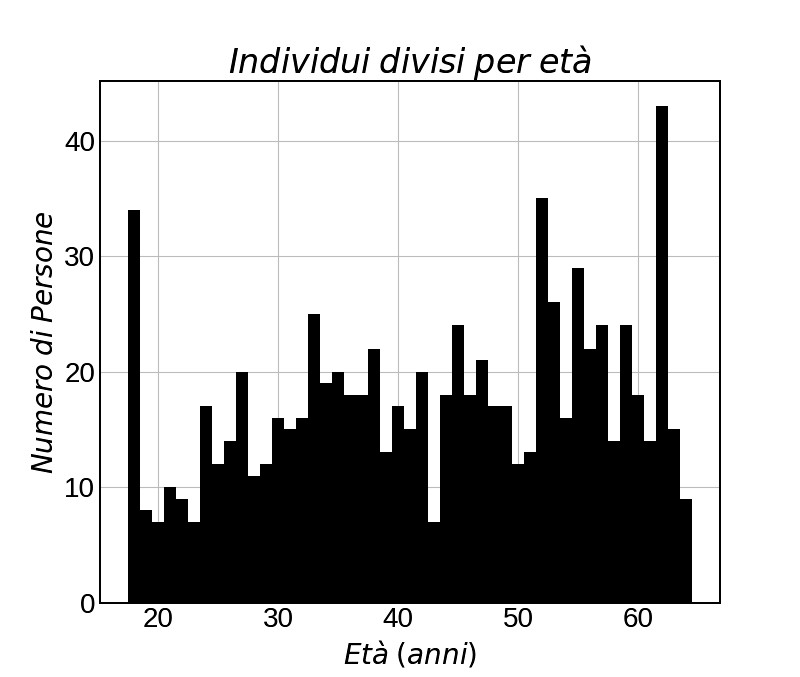
\includegraphics[width=\textwidth]{campione-age.jpg}
	\caption{Nel grafico viene mostrata la composizione del campione di persone analizzato, ovvero il numero di individui appartenenti ad ogni età.
Si vuole sottolineare che minore sarà il numero di occorrenze, maggiore sarà l'importanza dei singoli individui appartenenti a quella specifica età.
Pertanto si potranno osservare fluttuazioni brusche negli andamenti dei parametri sotto riportati, in quanto la presenza di un parametro fuori norma avrà peso maggiore per quei valori di età poco popolati.}
	\label{fig:campione-age}
\end{figure}


Con le features estratte si è potuto passare alla fase di analisi dati al fine di evidenziare differenze nel campione analizzato.
Prima di iniziare l'esposizione dei risultati ottenuti si vuole sottolineare come inevitabilmente il numero di individui influenzi la precisione dell'analisi ogniqualvolta si parli di statistica.
Pertanto certe brusche variazioni negli andamenti e nei grafici di questa sezione sono con buona probabilità da ricondursi al numero di individui che compongono il campione o il sotto-campione in questione. In Fig: \ref{fig:campione-age} viene mostrato il numero esatto di individui appartenenti ad ogni età tra 18 e 64 anni.



\subsection{Grafici riassuntivi sulla variazione delle features in funzione dell'età}

\begin{figure}[h!]
	\centering
	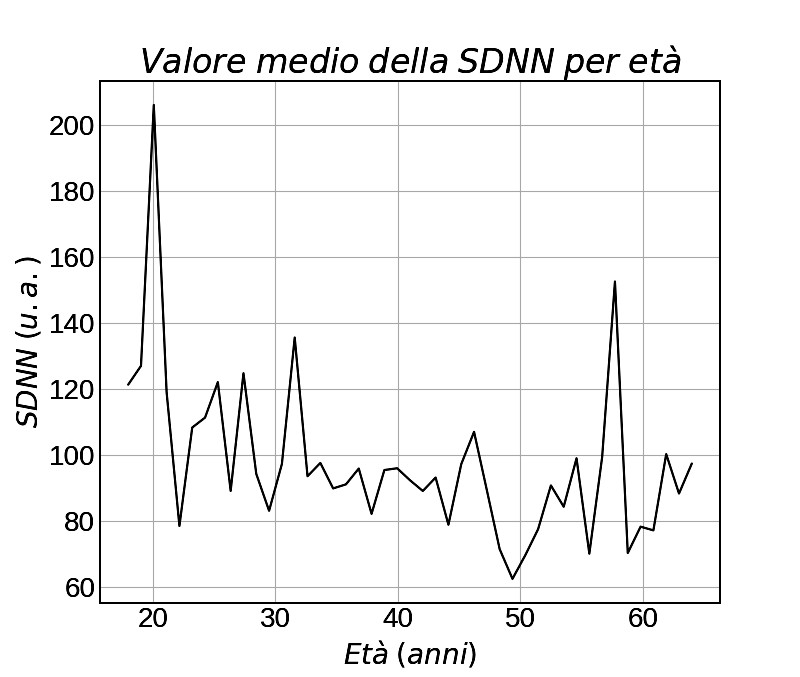
\includegraphics[width=\textwidth]{SDNN-age.jpg}
	\caption{Nel grafico viene mostrato il valore medio delle standard deviation 				effettuate sugli array $RR$ per ogni età presente nel database analizzato.
	Si noti come per questa feature (così come per altre) non vi siano andamenti 				apprezzabili che emergano al variare dell'età.}
	\label{fig:SDNN-age}
\end{figure}

\begin{figure}[h!]
	\centering
	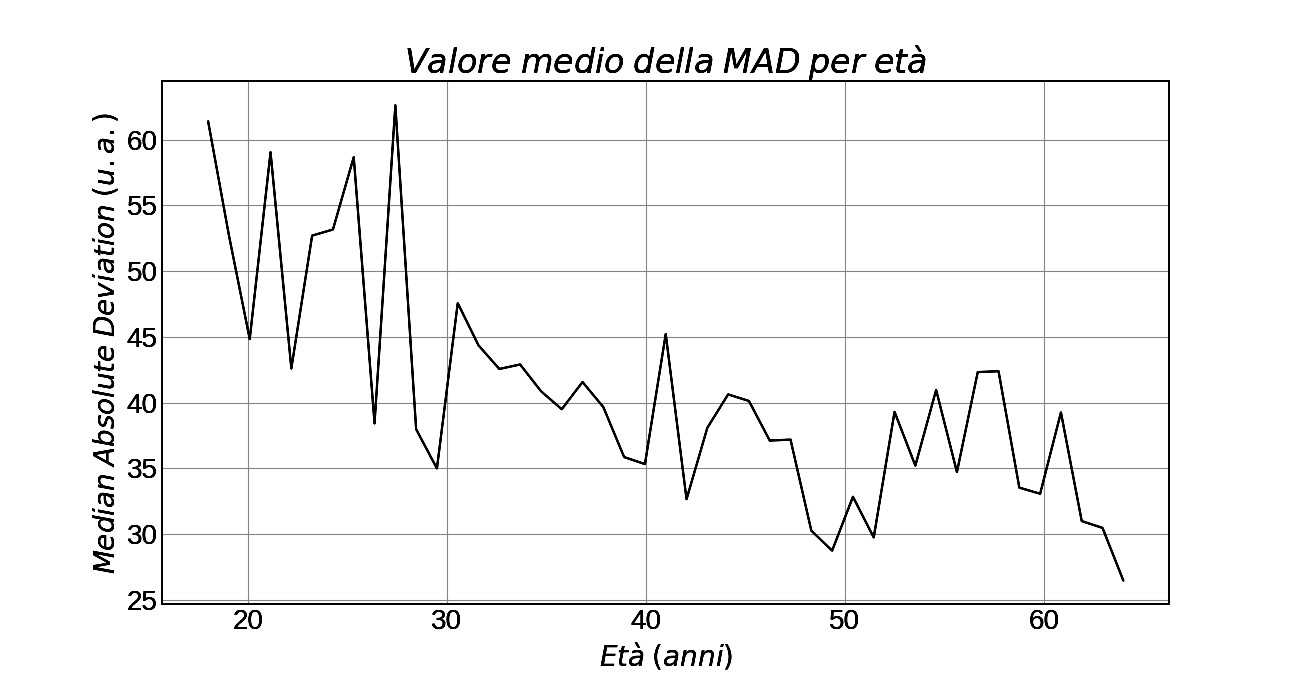
\includegraphics[width=\textwidth]{MAD-age.jpg}
	\caption{Nel grafico viene mostrato il valore medio della median absolute deviation 	per ogni età degli individui di appartenenza.
	Si noti come, nonostante le oscillazioni dovute ad un non elevato numero di 				campioni, tale parametro tenda a diminuire con l'età.}
	\label{fig:MAD-age}
\end{figure}

\begin{figure}[h!]
	\centering
	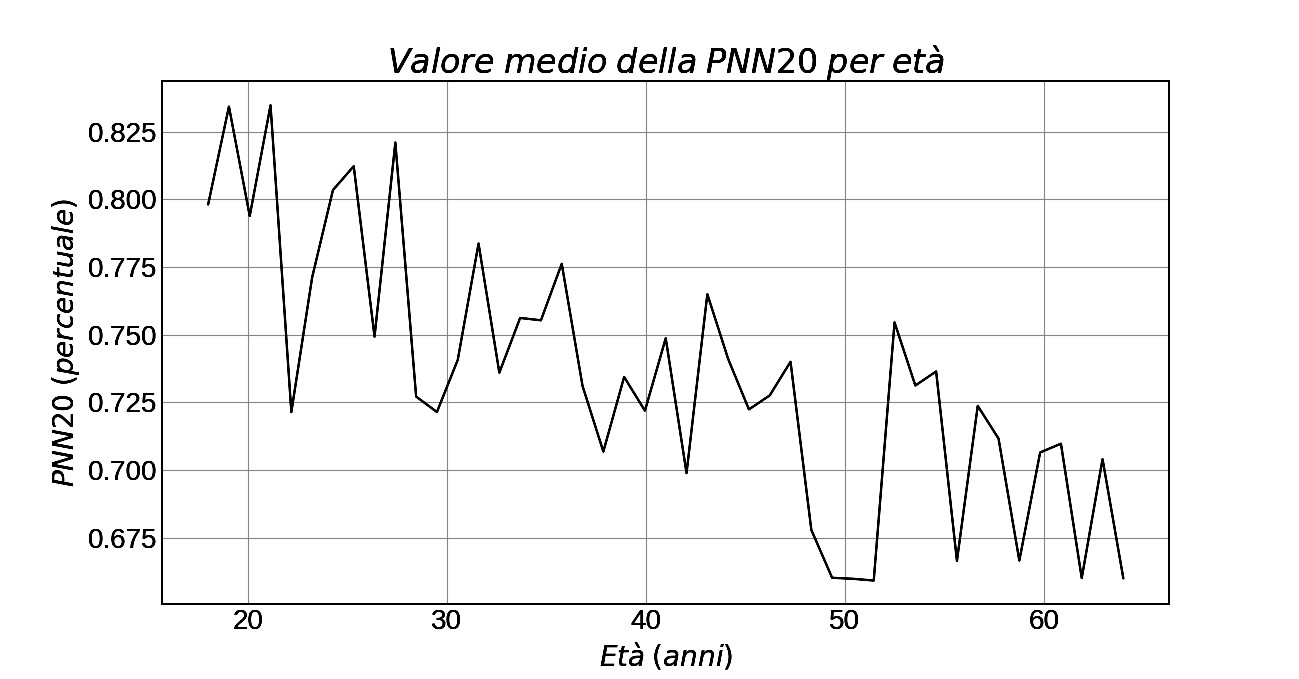
\includegraphics[width=\textwidth]{PNN20-age.jpg}
	\caption{Nel grafico viene mostrato il valore medio della PNN20 (ovvero la 					percentuale degli elementi di $RR_{diff}$ maggiore di $20ms$) per ogni età presente 	nel campione analizzato.
	Anche per questo parametro è possibile osservare una tendenza a diminuire con 				l'aumentare dell'età.}
	\label{fig:PNN20-age}
\end{figure}

\begin{figure}[h!]
	\centering
	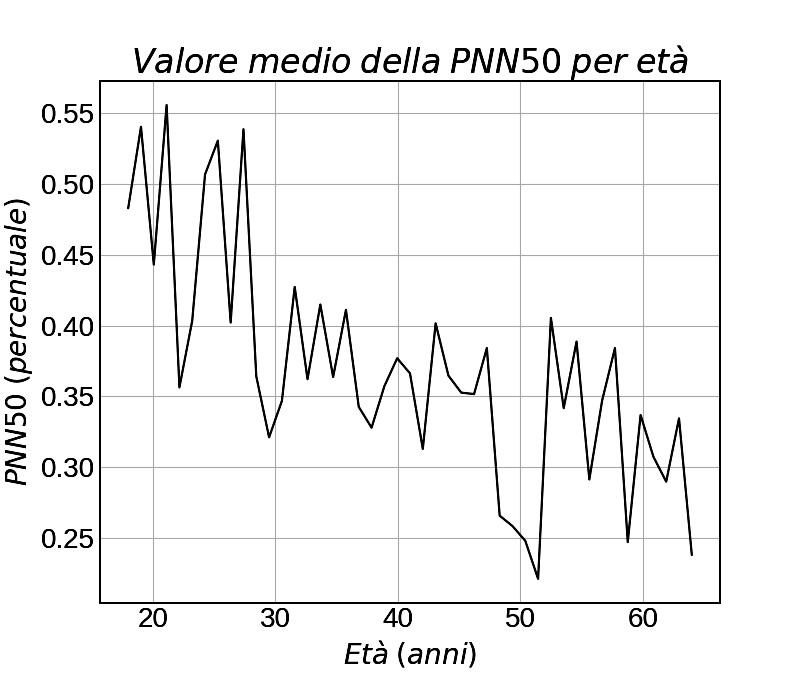
\includegraphics[width=\textwidth]{PNN50-age.jpg}
	\caption{Nel grafico viene mostrato il valore medio della PNN50 (ovvero la 					percentuale degli elementi di $RR_{diff}$ maggiore di $50ms$) per ogni età presente 	nel campione analizzato.
	Com'era prevedibile, vista la natura dei due parametri, si osserva un'andamento 			analogo a quello della $PNN20$, ossia una tendenza a diminuire con l'aumentare 				dell'età.}
	\label{fig:PNN50-age}
\end{figure}


Come è possibile notare la Fig: \ref{fig:SDNN-age} e la Fig: \ref{fig:MAD-age} differiscono nell'andamento mostrato nonostante siano entrambe indici di dispersione statistica.
Talle evento può essere fatto risalire al discorso iniziale dell'attuale capitolo ed alla maggior robustezza della MAD, già accennata nel precedente capitolo.
Gli andamenti in funzione dell'età di: MAD(Fig:\ref{fig:MAD-age}), PNN20(Fig:\ref{fig:PNN20-age}) e PNN50(Fig:\ref{fig:PNN50-age}) suggeriscono tutti una lieve ma rilevabile diminuzione della variabilità del ritmo cardiaco con l'età.


\subsection{Grafici comparativi tra diversi sotto-campioni}

\begin{figure}[h!]
	\centering
	\subfloat[Caratteristiche picco principale: $media=34.325$, $mediana=33.704$, $deviazione$ $standard=4.736$.]{\label{fig:mdleft}												{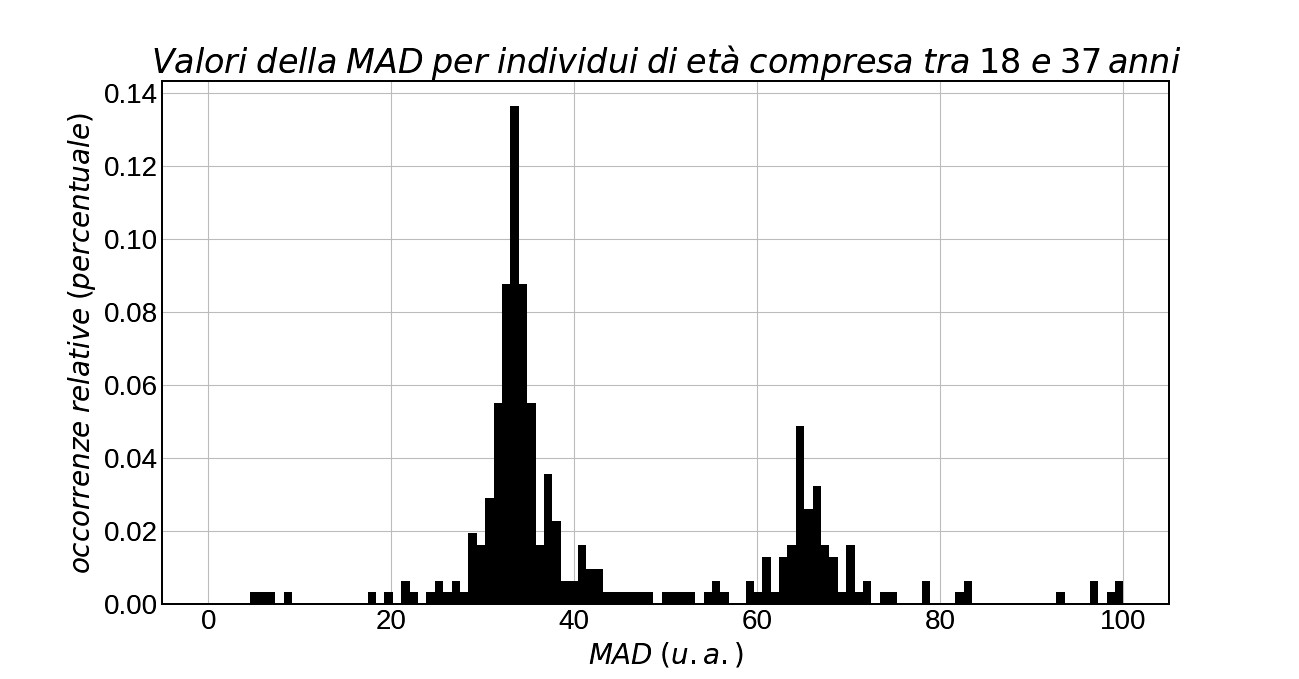
\includegraphics[width=\textwidth]{MAD-y.jpg}}}\hfill
	\subfloat[Caratteristiche picco principale: $media=31.535$, $mediana=32.187$, $deviazione$ $standard=4.802$.]{\label{fig:mdright}											{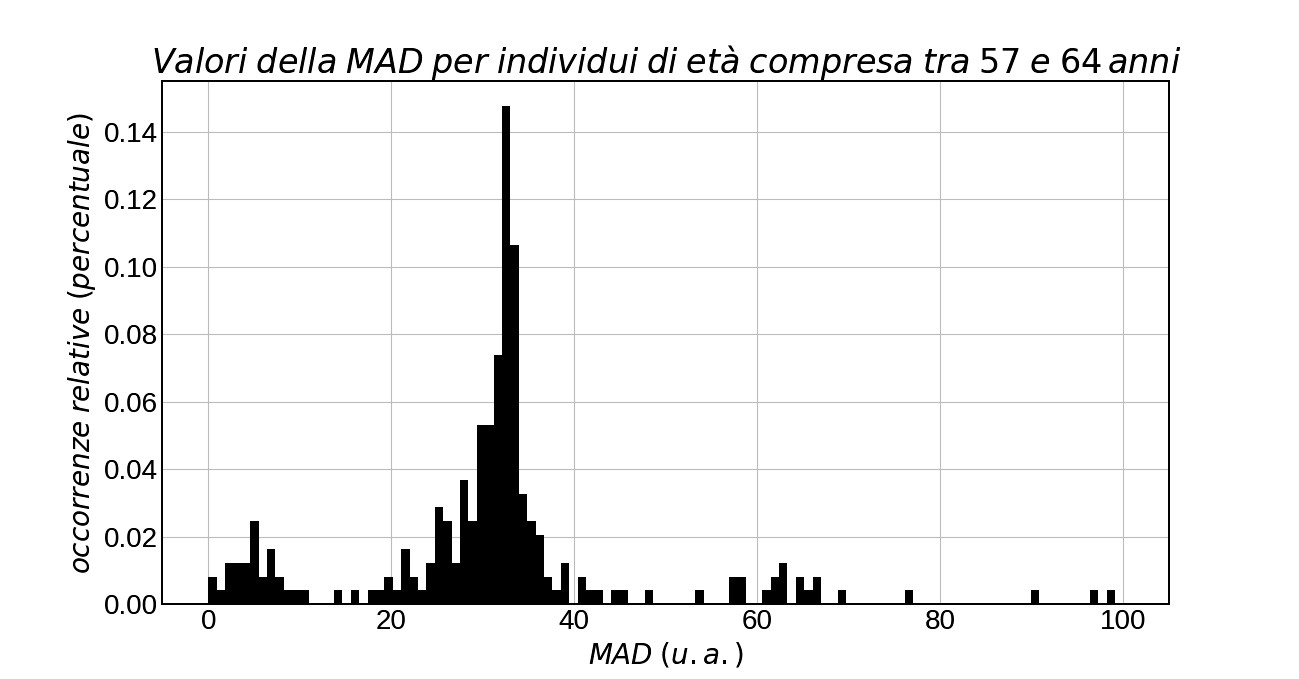
\includegraphics[width=\textwidth]{MAD-o.jpg}}}
	\caption{In figura è possibile confrontare la distribuzione della MAD raccolta da due campioni di età diverse.
	Le principali differenze consistono nella presenza di un picco avente MAD maggiore del picco principale nel campione più giovane (a) ed un picco avente MAD minore nel campione più anziano (b).
	Inoltre in (a) il 23.1\% del campione viene raccolto nel picco a MAD maggiore ed in (b) il 13.1\% viene raccolto nel picco a MAD minore.
	Risultano praticamente trascurabili il picco a MAD minore in (a) ed il picco a MAD maggiore in (b).}
	\label{fig:MAD}
\end{figure}

\begin{figure}[h!]
	\centering
	\subfloat[Caratteristiche della distribuzione: $media=0.593$, $mediana=0.604$, $deviazione$ $standard = 0.080$]{\label{fig:mdleft}												{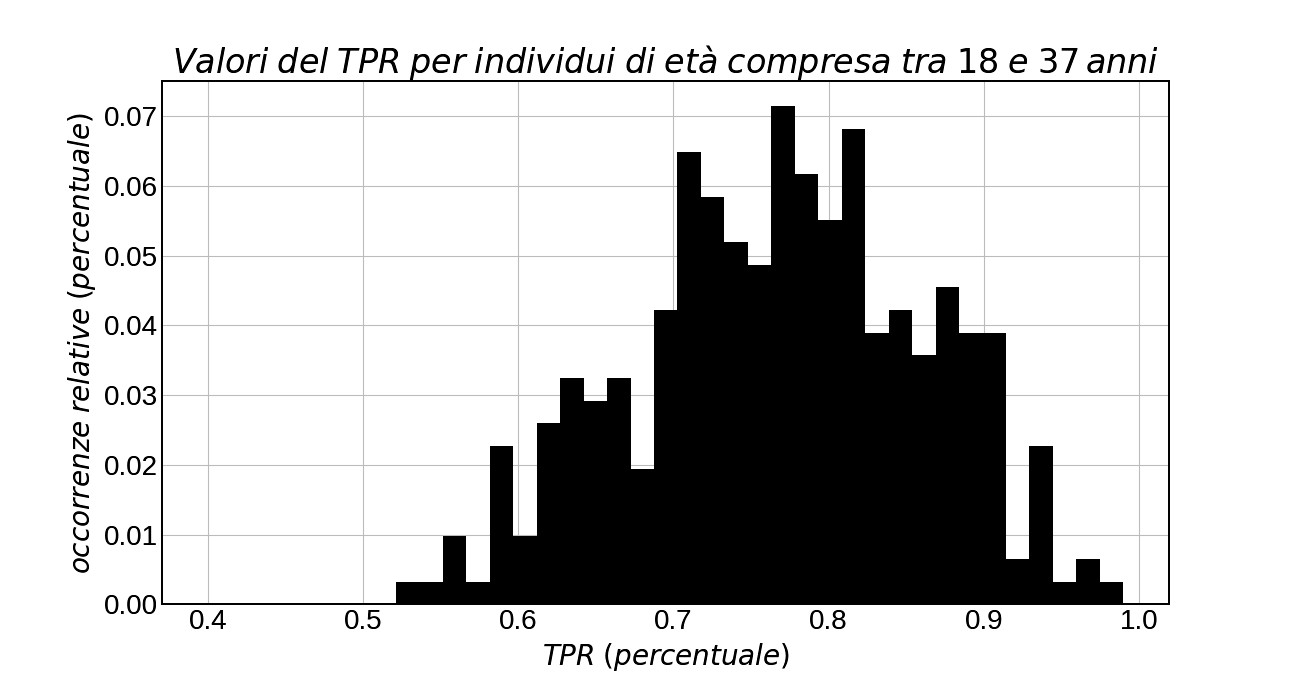
\includegraphics[width=\textwidth]{TPR-y.jpg}}}\hfill
	\subfloat[Caratteristiche della distribuzione: $media=0.668$, $mediana=0.681$, $deviazione$ $standard = 0.065$]{\label{fig:mdright}											{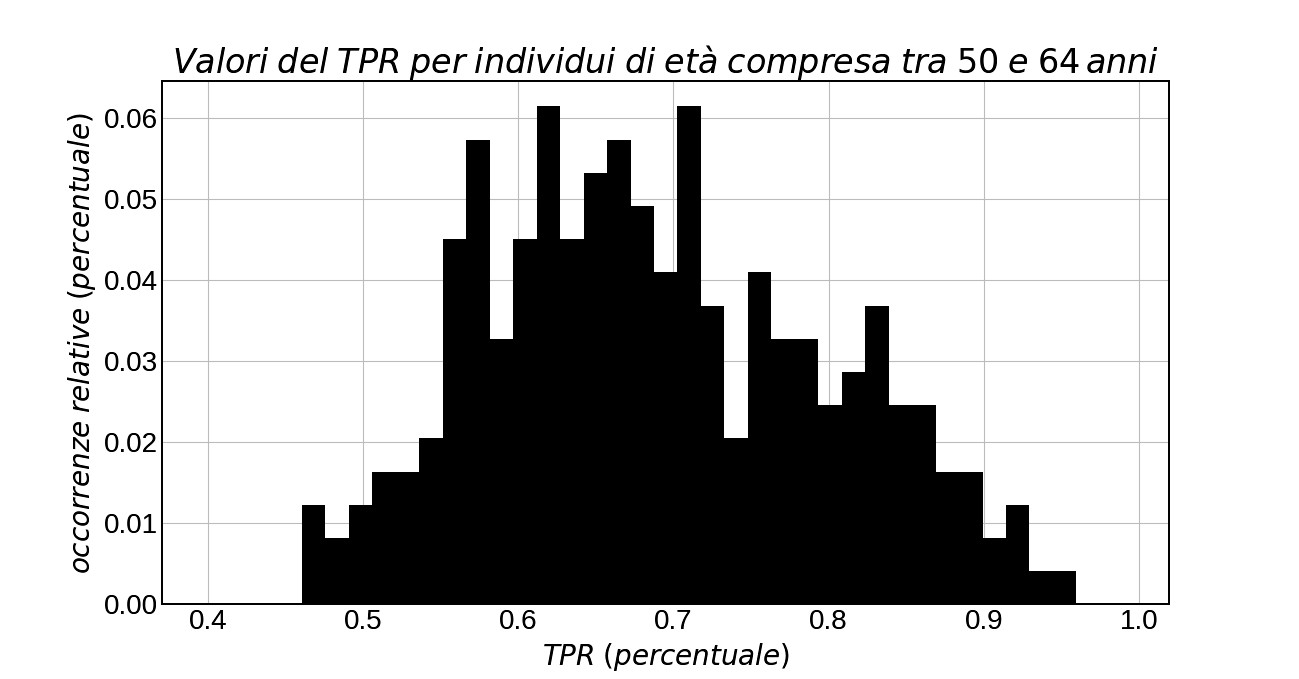
\includegraphics[width=\textwidth]{TPR-o.jpg}}}
	\caption{In figura è possibile confrontare il parametro TPR estratto da un campione giovane (a) ed un campione anziano (b).
	La principale differenza si nota a livello di media e mediana, dove lo scostamento tre le due distribuzioni appare numericamente evidente.}
	\label{fig:TPR}
\end{figure}

\begin{figure}[h!]
	\centering
	\subfloat[Caratteristiche della distribuzione: $media=0.768$, $mediana=0.771$, $deviazione$ $standard = 0.094$]{\label{fig:mdleft}												{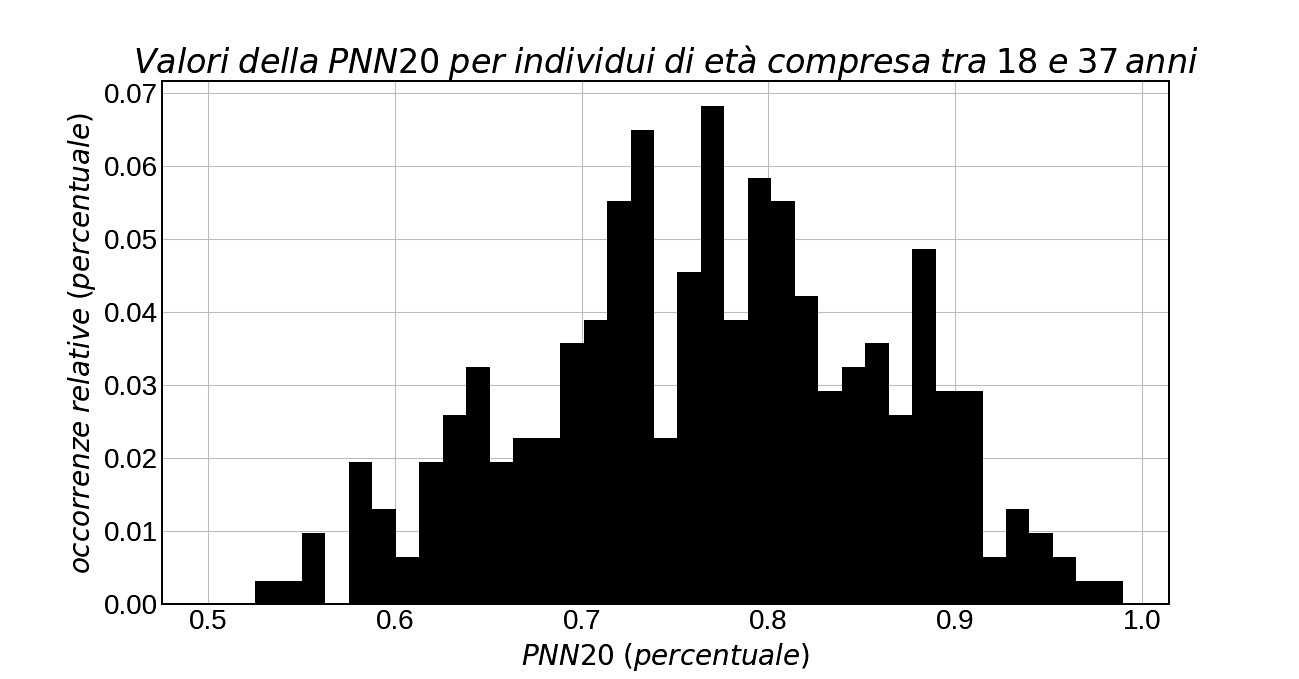
\includegraphics[width=\textwidth]{PNN20-y.jpg}}}\hfill
	\subfloat[Caratteristiche della distribuzione: $media=0.689$, $mediana=0.678$, $deviazione$ $standard = 0.109$]{\label{fig:mdright}						{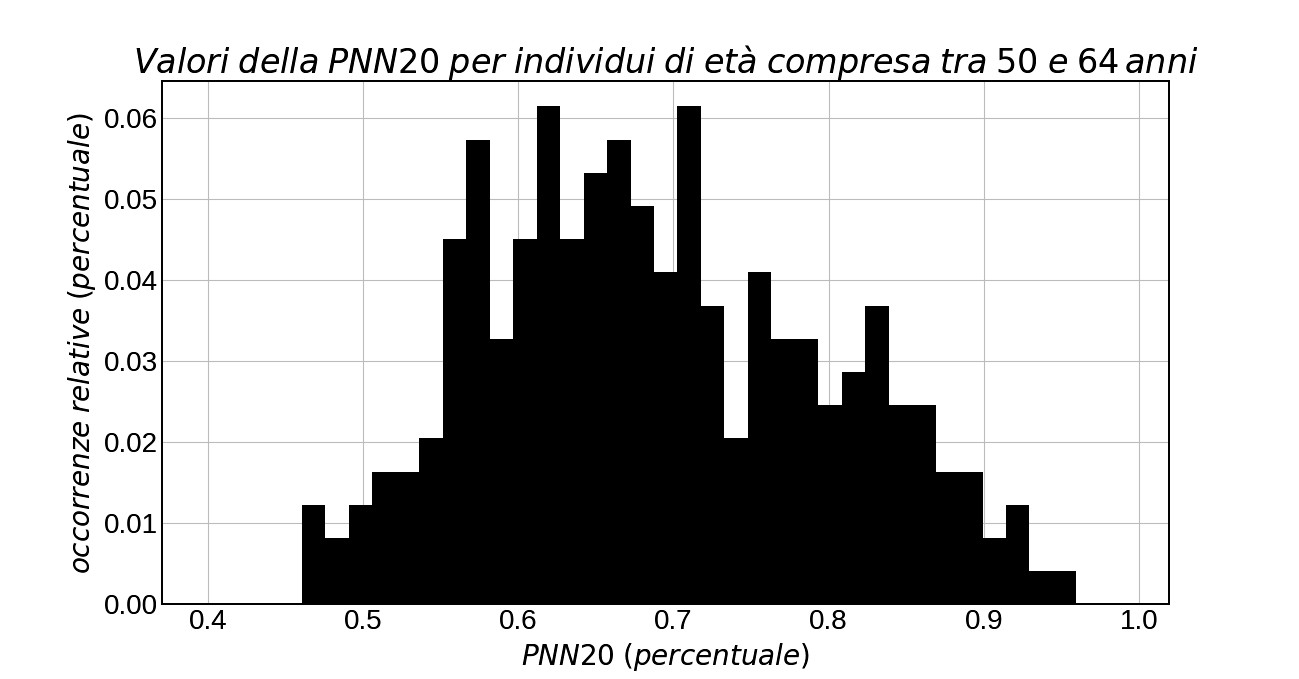
\includegraphics[width=\textwidth]{PNN20-o.jpg}}}
	\caption{In figura è possibile confrontare il parametro PNN20 estratto da un campione giovane (a) ed un campione anziano (b).
	La principale differenza tra le due distribuzioni risiede nella media e nella mediana.}
	\label{fig:PNN20}
\end{figure}

\begin{figure}[h!]
	\centering
	\subfloat[Caratteristiche della distribuzione: $media=0.422$, $mediana=0.420$, $deviazione$ $standard = 0.184$]{\label{fig:mdleft}												{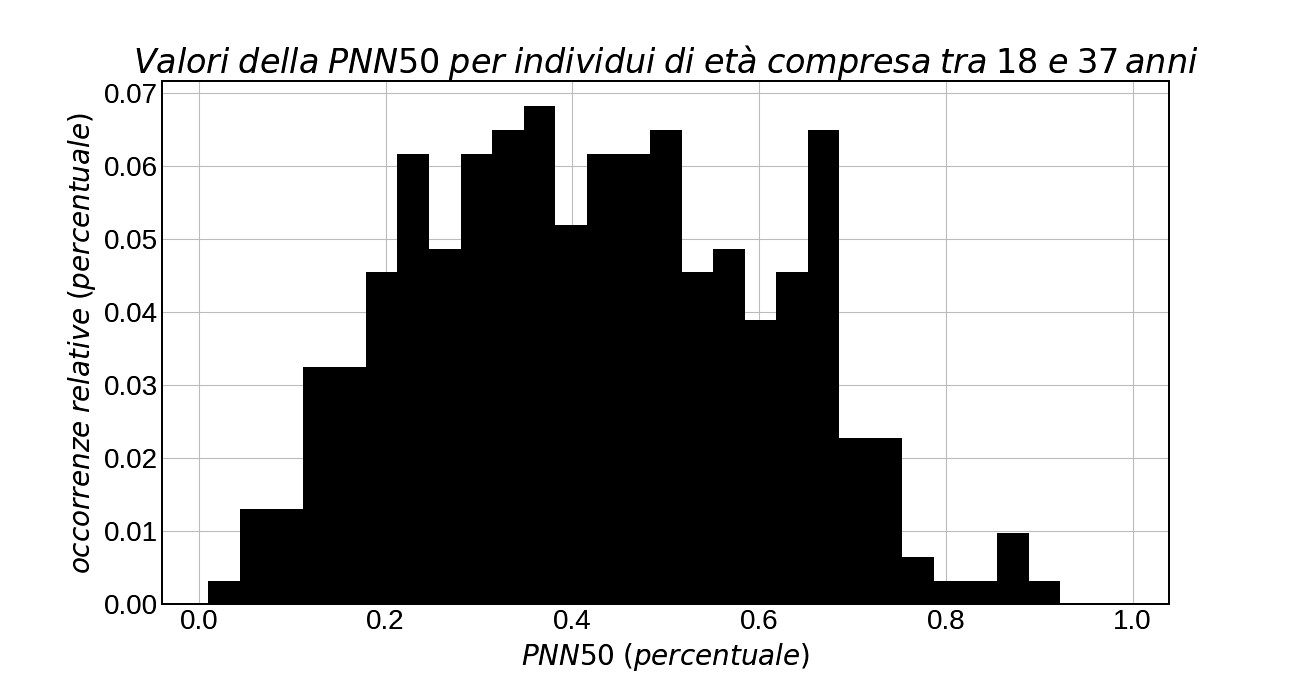
\includegraphics[width=\textwidth]{PNN50-y.jpg}}}\hfill
	\subfloat[Caratteristiche della distribuzione: $media=0.307$, $mediana=0.238$, $deviazione$ $standard = 0.206$]{\label{fig:mdright}											{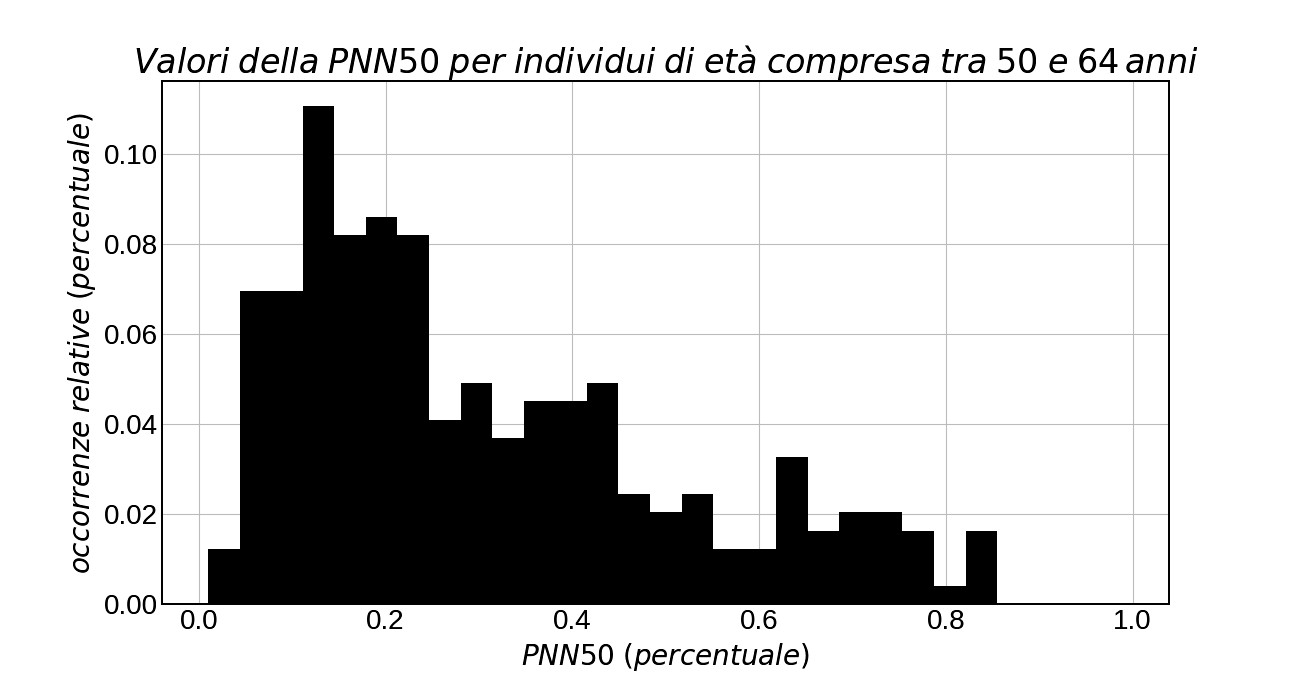
\includegraphics[width=\textwidth]{PNN50-o.jpg}}}
	\caption{In figura è possibile confrontare il parametro PNN50, anch'esso estratto da un campione giovane (a) ed un campione anziano (b).
	La principale differenza si nota sempre a livello di media e soprattutto a livello di mediana mediana, dove lo scostamento tre le due distribuzioni appare più accentuato.}
	\label{fig:PNN50}
\end{figure}

\begin{figure}[h!]
	\centering
	\subfloat[Caratteristiche della distribuzione: $media=1059ms$, $mediana=919ms$, $deviazione$ $standard = 758ms$]{\label{fig:mdleft}												{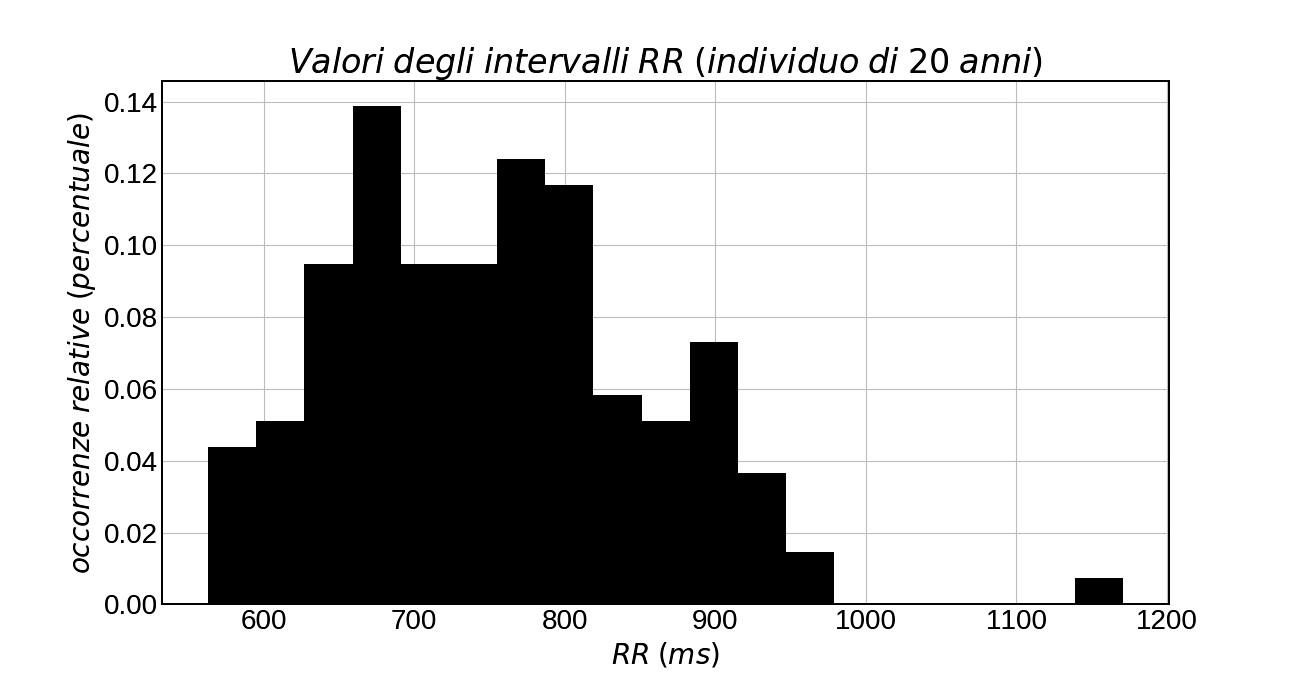
\includegraphics[width=\textwidth]{RR-20anni.jpg}}}\hfill
	\subfloat[Caratteristiche della distribuzione: $media=768ms$, $mediana=771ms$, $deviazione$ $standard = 94.2ms$]{\label{fig:mdright}											{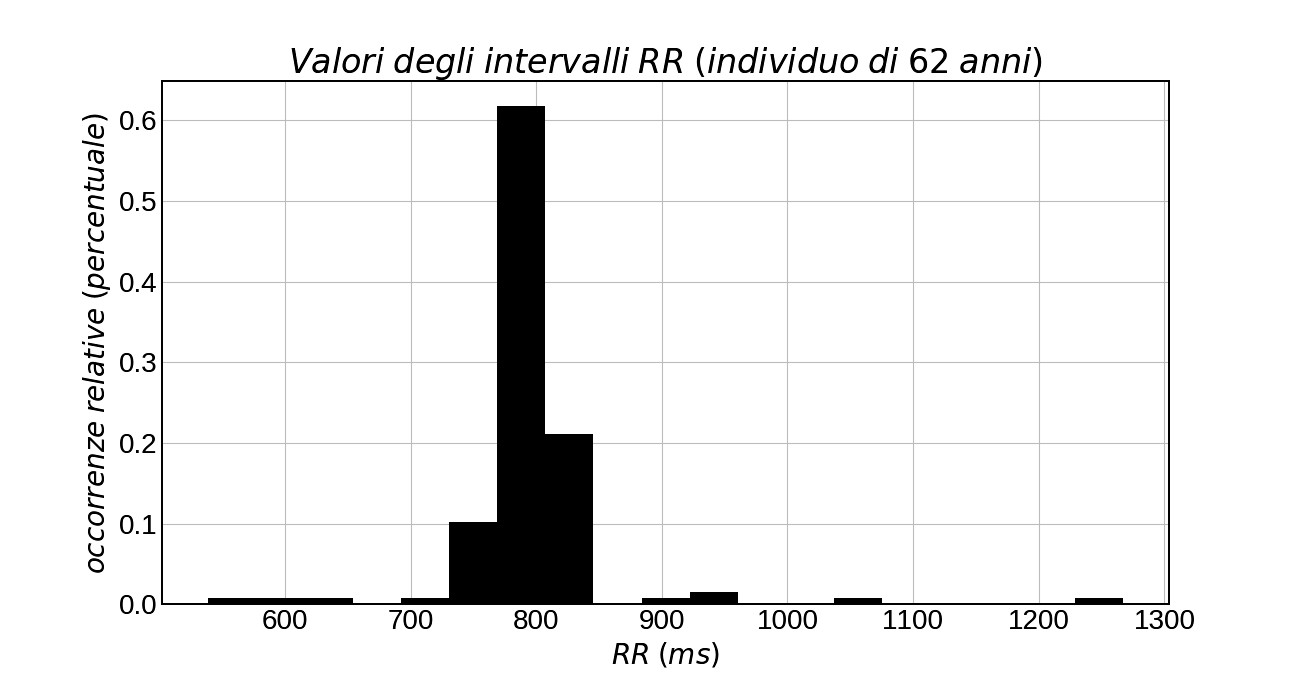
\includegraphics[width=\textwidth]{RR-62anni.jpg}}}
	\caption{Qui sono messi a confronto i valori degli intervalli RR per un soggetto giovane (a) (20 anni) ed uno meno giovane (b) (62 anni).
	Non si può dare peso alla differenza di media, in quanto ogni individuo ha la propria e questa stessa è a sua volta molto variabile a seconda di cosa si stia facendo, Spicca però la notevole differenza tra le deviazioni standard, ad indicare che per un individuo giovane si ha una maggiore variabilità negli intervalli RR di quanto non si abbia in un individuo più anziano.}
	\label{fig:RR_y_vs_o}
\end{figure}


La diminuzione della media della distribuzione del TPR (FIG:\ref{fig:TPR}) suggerisce una minor casualità all'interno degli intervalli tra picchi R con l'invecchiamento.
Le diminuzioni considerevoli delle mediane per le distribuzioni di PNN20 (Fig:\ref{fig:PNN20}) e PNN50 (Fig:\ref{fig:PNN50}) dimostrano una minore variabilità nel ritmo cardiaco per il campione più anziano e tali effetti sono ancora più visibili nella differenza tra le deviazioni standard degli array RR mostrati in Fig:\ref{fig:RR_y_vs_o}.
Infine nella MAD si osservano tre picchi: il primo (compreso tra 0 e 20 u.a.) si manifesta esclusivamente per campioni più anziani, il secondo (compreso tra 20 e 60 u.a.) è il maggiore ed è sempre presente, il terzo (compreso tra 60 ed 80 u.a.) è visibile solo per campioni più giovani. 
Dunque anche i grafici comparativi mostrano una diminuzione della heart rate variability e della complessità del segnale come conseguenza dell'invecchiamento.



\chapter{Conclusioni}



Alcuni indicatori di dispersione come MAD, PNN20 e PNN50 hanno mostrato un calo con l'aumentare dell'età.
Il fatto che la deviazione standard non abbia evidenziato alcun tipo di andamento può esser fatto risalire allo scarso numero di campioni impiegati, i quali avrebbero reso eccessivamente influenti i pochi a disposizione.
È stato dunque importante introdurre la MAD, in quanto più robusta contro questo tipo di problemi e dunque più affidabile nel nostro caso.
Il calo del TPR avvenuto con l'aumentare dell'età può essere visto sia come minor casualità della serie temporale, sia come minor complessità del segnale analizzato. 
In conclusione si evidenzia una diminuzione di complessità e variabilità del ritmo cardiaco tra soggetti più giovani e soggetti più anziani.
Tale fatto concorda con la letteratura attualmente a disposizione e suggerisce l'importanza ancora non pienamente compresa della heart rate variability per un soggetto in salute.



\chapter*{Appendici}



\section*{Appendice A}


\subsection{dimostrazione della legge di Lambert-Beer}

Si può derivare la legge di attenuazione dell'intensità luminosa di un fascio di radiazione elettromagnetica monocromatica con intensità iniziale $I_0$ dalle seguenti assunzioni:\begin{itemize}
    \item si suppone che il fascio viaggi parallelo ad un asse di riferimento $x$;
    \item si suppone che si possa definire una intensità locale funzione della distanza 		  $I = I(x)$;
    \item si suppone che l'attenuazione di intensità $dI$ sia proporzionale 						  all'intensità $I$, alla concentrazione molare del campione $C$ ed al cammino 				  infinitesimo $dx$ attraverso un certo coefficiente $\varepsilon_{\lambda}^{'}				  $.
\end{itemize}
Dunque si ha la seguente relazione differenziale
\begin{equation*}
    dI = -\varepsilon_{\lambda}CI dx
\end{equation*}
integrando l'equazione differenziale a variabili separabili si ottiene
\begin{equation*}
    ln(\frac{I}{I_0}) = -\varepsilon_{\lambda}Cl
\end{equation*}
ed infine
\begin{equation*}
    I = I_0e^{-\varepsilon_{\lambda}Cl} = I_010^{-\varepsilon_{\lambda}^{'}Cl}
\end{equation*}
dove $\varepsilon_{\lambda}^{'} = \frac{\varepsilon_{\lambda}}{ln(10)}$ .




\thispagestyle{empty}
\newpage
\thispagestyle{empty}



\begin{thebibliography}{1}
\bibitem{Pulseoximeter}
Edward D. Chan, Michael M. Chan, Mallory M. Chan. 
\textit{Pulse oximetry: Understanding its basic principles facilitates appreciation of its limitations}. 
Respiratory Medicine. Anno: 2013. Pag. 789-791
\\\texttt{https://www.boxym.com/wp-content/uploads/2018/07/Pulse-oximetry-Understanding-its-basic-principles-facilitates-appreciation-of-its-limitations.pdf}


\bibitem{Sickle}
Ortiz FO, Aldrich TK, Nagel RL, Benjamin LJ.
\textit{Accuracy of pulseoximetry in sickle cell disease.}
Am J Respir Crit Care Med. Anno: 1999. pag. 159-447 e 51.


\bibitem{Hemoglobin}
Ranjan K. Dash and James B. Bassingthwaighte
\textit{Erratum to: Blood HbO2 and HbCO2 Dissociation Curves at Varied O2, CO2, pH, 2,3-DPG and Temperature Levels}.
Ann Biomeg Eng. Anno: 2010 Apr; 38(4): 1683–1701. 
\\\texttt{https://www.ncbi.nlm.nih.gov/pmc/articles/PMC2862600/}


\bibitem{Afib}
Tang SC, et al. 
\textit{Identification of Atrial Fibrillation by Quantitative Analyses of Fingertip Photoplethysmogram.} Sci Rep. 2017;7:45644. doi: 10.1038/srep45644.


\bibitem{HRV}
Daniel T. Kaplan, et al.
\textit{Aging and the complexity of cardiovascular dynamics.}
Biophysical journal. Volume 59. Anno:1991 Apr. pag.945-949



\end{thebibliography}


\end{document}